\documentclass{article}
\usepackage{onecolceurws}
\usepackage{amssymb}
\usepackage{mathabx}
\usepackage{subcaption}
\usepackage{graphicx}
%% ODER: format ==         = "\mathrel{==}"
%% ODER: format /=         = "\neq "
%
%
\makeatletter
\@ifundefined{lhs2tex.lhs2tex.sty.read}%
  {\@namedef{lhs2tex.lhs2tex.sty.read}{}%
   \newcommand\SkipToFmtEnd{}%
   \newcommand\EndFmtInput{}%
   \long\def\SkipToFmtEnd#1\EndFmtInput{}%
  }\SkipToFmtEnd

\newcommand\ReadOnlyOnce[1]{\@ifundefined{#1}{\@namedef{#1}{}}\SkipToFmtEnd}
\usepackage{amstext}
\usepackage{amssymb}
\usepackage{stmaryrd}
\DeclareFontFamily{OT1}{cmtex}{}
\DeclareFontShape{OT1}{cmtex}{m}{n}
  {<5><6><7><8>cmtex8
   <9>cmtex9
   <10><10.95><12><14.4><17.28><20.74><24.88>cmtex10}{}
\DeclareFontShape{OT1}{cmtex}{m}{it}
  {<-> ssub * cmtt/m/it}{}
\newcommand{\texfamily}{\fontfamily{cmtex}\selectfont}
\DeclareFontShape{OT1}{cmtt}{bx}{n}
  {<5><6><7><8>cmtt8
   <9>cmbtt9
   <10><10.95><12><14.4><17.28><20.74><24.88>cmbtt10}{}
\DeclareFontShape{OT1}{cmtex}{bx}{n}
  {<-> ssub * cmtt/bx/n}{}
\newcommand{\tex}[1]{\text{\texfamily#1}}	% NEU

\newcommand{\Sp}{\hskip.33334em\relax}


\newcommand{\Conid}[1]{\mathit{#1}}
\newcommand{\Varid}[1]{\mathit{#1}}
\newcommand{\anonymous}{\kern0.06em \vbox{\hrule\@width.5em}}
\newcommand{\plus}{\mathbin{+\!\!\!+}}
\newcommand{\bind}{\mathbin{>\!\!\!>\mkern-6.7mu=}}
\newcommand{\rbind}{\mathbin{=\mkern-6.7mu<\!\!\!<}}% suggested by Neil Mitchell
\newcommand{\sequ}{\mathbin{>\!\!\!>}}
\renewcommand{\leq}{\leqslant}
\renewcommand{\geq}{\geqslant}
\usepackage{polytable}

%mathindent has to be defined
\@ifundefined{mathindent}%
  {\newdimen\mathindent\mathindent\leftmargini}%
  {}%

\def\resethooks{%
  \global\let\SaveRestoreHook\empty
  \global\let\ColumnHook\empty}
\newcommand*{\savecolumns}[1][default]%
  {\g@addto@macro\SaveRestoreHook{\savecolumns[#1]}}
\newcommand*{\restorecolumns}[1][default]%
  {\g@addto@macro\SaveRestoreHook{\restorecolumns[#1]}}
\newcommand*{\aligncolumn}[2]%
  {\g@addto@macro\ColumnHook{\column{#1}{#2}}}

\resethooks

\newcommand{\onelinecommentchars}{\quad-{}- }
\newcommand{\commentbeginchars}{\enskip\{-}
\newcommand{\commentendchars}{-\}\enskip}

\newcommand{\visiblecomments}{%
  \let\onelinecomment=\onelinecommentchars
  \let\commentbegin=\commentbeginchars
  \let\commentend=\commentendchars}

\newcommand{\invisiblecomments}{%
  \let\onelinecomment=\empty
  \let\commentbegin=\empty
  \let\commentend=\empty}

\visiblecomments

\newlength{\blanklineskip}
\setlength{\blanklineskip}{0.66084ex}

\newcommand{\hsindent}[1]{\quad}% default is fixed indentation
\let\hspre\empty
\let\hspost\empty
\newcommand{\NB}{\textbf{NB}}
\newcommand{\Todo}[1]{$\langle$\textbf{To do:}~#1$\rangle$}

\EndFmtInput
\makeatother
%
%
%
%
%
%
% This package provides two environments suitable to take the place
% of hscode, called "plainhscode" and "arrayhscode". 
%
% The plain environment surrounds each code block by vertical space,
% and it uses \abovedisplayskip and \belowdisplayskip to get spacing
% similar to formulas. Note that if these dimensions are changed,
% the spacing around displayed math formulas changes as well.
% All code is indented using \leftskip.
%
% Changed 19.08.2004 to reflect changes in colorcode. Should work with
% CodeGroup.sty.
%
\ReadOnlyOnce{polycode.fmt}%
\makeatletter

\newcommand{\hsnewpar}[1]%
  {{\parskip=0pt\parindent=0pt\par\vskip #1\noindent}}

% can be used, for instance, to redefine the code size, by setting the
% command to \small or something alike
\newcommand{\hscodestyle}{}

% The command \sethscode can be used to switch the code formatting
% behaviour by mapping the hscode environment in the subst directive
% to a new LaTeX environment.

\newcommand{\sethscode}[1]%
  {\expandafter\let\expandafter\hscode\csname #1\endcsname
   \expandafter\let\expandafter\endhscode\csname end#1\endcsname}

% "compatibility" mode restores the non-polycode.fmt layout.

\newenvironment{compathscode}%
  {\par\noindent
   \advance\leftskip\mathindent
   \hscodestyle
   \let\\=\@normalcr
   \let\hspre\(\let\hspost\)%
   \pboxed}%
  {\endpboxed\)%
   \par\noindent
   \ignorespacesafterend}

\newcommand{\compaths}{\sethscode{compathscode}}

% "plain" mode is the proposed default.
% It should now work with \centering.
% This required some changes. The old version
% is still available for reference as oldplainhscode.

\newenvironment{plainhscode}%
  {\hsnewpar\abovedisplayskip
   \advance\leftskip\mathindent
   \hscodestyle
   \let\hspre\(\let\hspost\)%
   \pboxed}%
  {\endpboxed%
   \hsnewpar\belowdisplayskip
   \ignorespacesafterend}

\newenvironment{oldplainhscode}%
  {\hsnewpar\abovedisplayskip
   \advance\leftskip\mathindent
   \hscodestyle
   \let\\=\@normalcr
   \(\pboxed}%
  {\endpboxed\)%
   \hsnewpar\belowdisplayskip
   \ignorespacesafterend}

% Here, we make plainhscode the default environment.

\newcommand{\plainhs}{\sethscode{plainhscode}}
\newcommand{\oldplainhs}{\sethscode{oldplainhscode}}
\plainhs

% The arrayhscode is like plain, but makes use of polytable's
% parray environment which disallows page breaks in code blocks.

\newenvironment{arrayhscode}%
  {\hsnewpar\abovedisplayskip
   \advance\leftskip\mathindent
   \hscodestyle
   \let\\=\@normalcr
   \(\parray}%
  {\endparray\)%
   \hsnewpar\belowdisplayskip
   \ignorespacesafterend}

\newcommand{\arrayhs}{\sethscode{arrayhscode}}

% The mathhscode environment also makes use of polytable's parray 
% environment. It is supposed to be used only inside math mode 
% (I used it to typeset the type rules in my thesis).

\newenvironment{mathhscode}%
  {\parray}{\endparray}

\newcommand{\mathhs}{\sethscode{mathhscode}}

% texths is similar to mathhs, but works in text mode.

\newenvironment{texthscode}%
  {\(\parray}{\endparray\)}

\newcommand{\texths}{\sethscode{texthscode}}

% The framed environment places code in a framed box.

\def\codeframewidth{\arrayrulewidth}
\RequirePackage{calc}

\newenvironment{framedhscode}%
  {\parskip=\abovedisplayskip\par\noindent
   \hscodestyle
   \arrayrulewidth=\codeframewidth
   \tabular{@{}|p{\linewidth-2\arraycolsep-2\arrayrulewidth-2pt}|@{}}%
   \hline\framedhslinecorrect\\{-1.5ex}%
   \let\endoflinesave=\\
   \let\\=\@normalcr
   \(\pboxed}%
  {\endpboxed\)%
   \framedhslinecorrect\endoflinesave{.5ex}\hline
   \endtabular
   \parskip=\belowdisplayskip\par\noindent
   \ignorespacesafterend}

\newcommand{\framedhslinecorrect}[2]%
  {#1[#2]}

\newcommand{\framedhs}{\sethscode{framedhscode}}

% The inlinehscode environment is an experimental environment
% that can be used to typeset displayed code inline.

\newenvironment{inlinehscode}%
  {\(\def\column##1##2{}%
   \let\>\undefined\let\<\undefined\let\\\undefined
   \newcommand\>[1][]{}\newcommand\<[1][]{}\newcommand\\[1][]{}%
   \def\fromto##1##2##3{##3}%
   \def\nextline{}}{\) }%

\newcommand{\inlinehs}{\sethscode{inlinehscode}}

% The joincode environment is a separate environment that
% can be used to surround and thereby connect multiple code
% blocks.

\newenvironment{joincode}%
  {\let\orighscode=\hscode
   \let\origendhscode=\endhscode
   \def\endhscode{\def\hscode{\endgroup\def\@currenvir{hscode}\\}\begingroup}
   %\let\SaveRestoreHook=\empty
   %\let\ColumnHook=\empty
   %\let\resethooks=\empty
   \orighscode\def\hscode{\endgroup\def\@currenvir{hscode}}}%
  {\origendhscode
   \global\let\hscode=\orighscode
   \global\let\endhscode=\origendhscode}%

\makeatother
\EndFmtInput
%

\def\comment#1{$\Rightarrow$ {\em #1} $\Leftarrow$}

\renewcommand{\paragraph}[1]{\vspace{0.2cm}\noindent {\bf #1} $\;\;$}

% ------------------------------------------------------------------------------
% - title and stuff

\title{Handling Common Transitive Relations\\in First-Order Automated Reasoning}

%\titlerunning{Handling Common Transitive Relations}

\author{
  Koen Claessen
  \and 
  Ann Lilliestr{\"o}m
}

%\authorrunning{Claessen, Lilliestr{\"o}m}

\institution{
  Chalmers University of Technology\\
  {\sf \{koen,annl\}@chalmers.se}
}

\begin{document}

\maketitle

% ------------------------------------------------------------------------------
% - some symbols












% ------------------------------------------------------------------------------
% - abstract

\begin{abstract}
We present a number of alternative ways of handling transitive binary relations that commonly occur in first-order problems, in particular {\em equivalence relations}, {\em total orders}, and {\em reflexive, transitive relations}. We show how such relations can be discovered syntactically in an input theory. We experimentally evaluate different treatments on problems from the TPTP, using resolution-based reasoning tools as well as instance-based tools. Our conclusions are that (1) it is beneficial to consider different treatments of binary relations as a user, and that (2) reasoning tools could benefit from using a preprocessor or even built-in support for certain binary relations.
\end{abstract}

% ------------------------------------------------------------------------------
% - introduction

\section{Introduction}

Most automated reasoning tools for first-order logic have some kind of built-in support for reasoning about equality. Equality is one of the most common binary relations, and there are great performance benefits from providing built-in support for equality. Together, these two advantages by far outweigh the cost of implementation.

Other common concepts for which there exists built-in support in many tools are associative, commutative operators; and real-valued, rational-valued, and integer-valued arithmetic. Again, these concepts seem to appear often enough to warrant the extra cost of implementing special support in reasoning tools.

This paper is concerned with investigating what kind of special treatment we could give to commonly appearing transitive binary relations, and what effect this treatment has in practice. Adding special treatment of transitive relations to reasoning tools has been the subject of study before, in particular by means of {\em chaining} \cite{chaining}. The transitivity axiom
\begin{hscode}\SaveRestoreHook
\column{B}{@{}>{\hspre}l<{\hspost}@{}}%
\column{E}{@{}>{\hspre}l<{\hspost}@{}}%
\>[B]{}\forall{}\hspace{-0.1cm}\;\Varid{x},\Varid{y},\Varid{z}.\;R\hspace{-0.1cm}\;(\Varid{x},\Varid{y})\mathrel{\wedge}R\hspace{-0.1cm}\;(\Varid{y},\Varid{z})\Rightarrow R\hspace{-0.1cm}\;(\Varid{x},\Varid{z}){}\<[E]%
\ColumnHook
\end{hscode}\resethooks
can lead to an expensive proof exploration in resolution and superposition based theorem provers, and can generate a huge number of instances in instance-based provers and SMT-solvers. Transitive relations are also common enough to motivate special built-in support. However, as far as we know, chaining is not implemented in any of the major first-order reasoning tools (at least not in E \cite{E}, Vampire \cite{Vampire}, Z3 \cite{Z3}, and CVC4 \cite{CVC4}, which were used in this paper).

As an alternative to adding built-in support, in this paper we mainly look at (1) what a user of a reasoning tool may do herself to optimize the handling of these relations, and (2) how a preprocessing tool may be able to do this automatically. Adding built-in reasoning support in the tools themselves is not a main concern of this paper.

By ``treatment'' we mean any way of logically expressing the relation. For example, a possible treatment of a binary relation \ensuremath{R} in a theory \ensuremath{\Conid{T}} may simply mean axiomatizing \ensuremath{R} in \ensuremath{\Conid{T}}. But it may also mean transforming \ensuremath{\Conid{T}} into a satisfiability-equivalent theory \ensuremath{\Conid{T'}} where \ensuremath{R} does not even syntactically appear.

As an example, consider a theory \ensuremath{\Conid{T}} in which an equivalence relation \ensuremath{R} occurs. One way to deal with \ensuremath{R} is to simply axiomatize it, by means of reflexivity, symmetry, and transitivity:
\begin{hscode}\SaveRestoreHook
\column{B}{@{}>{\hspre}l<{\hspost}@{}}%
\column{15}{@{}>{\hspre}l<{\hspost}@{}}%
\column{E}{@{}>{\hspre}l<{\hspost}@{}}%
\>[B]{}\forall{}\hspace{-0.1cm}\;\Varid{x}{}\<[15]%
\>[15]{}.\;R\hspace{-0.1cm}\;(\Varid{x},\Varid{x}){}\<[E]%
\\
\>[B]{}\forall{}\hspace{-0.1cm}\;\Varid{x},\Varid{y}{}\<[15]%
\>[15]{}.\;R\hspace{-0.1cm}\;(\Varid{x},\Varid{y})\Rightarrow R\hspace{-0.1cm}\;(\Varid{y},\Varid{x}){}\<[E]%
\\
\>[B]{}\forall{}\hspace{-0.1cm}\;\Varid{x},\Varid{y},\Varid{z}{}\<[15]%
\>[15]{}.\;R\hspace{-0.1cm}\;(\Varid{x},\Varid{y})\mathrel{\wedge}R\hspace{-0.1cm}\;(\Varid{y},\Varid{z})\Rightarrow R\hspace{-0.1cm}\;(\Varid{x},\Varid{z}){}\<[E]%
\ColumnHook
\end{hscode}\resethooks
Another way is to ``borrow'' the built-in equality treatment that exists in most theorem provers. We can do this by introducing a new symbol \ensuremath{rep}, and replacing all occurrences of \ensuremath{R\hspace{-0.1cm}\;(\Varid{x},\Varid{y})} by the formula:
\begin{hscode}\SaveRestoreHook
\column{B}{@{}>{\hspre}l<{\hspost}@{}}%
\column{E}{@{}>{\hspre}l<{\hspost}@{}}%
\>[B]{}rep\hspace{-0.1cm}\;(\Varid{x})\mathrel{=}rep\hspace{-0.1cm}\;(\Varid{y}){}\<[E]%
\ColumnHook
\end{hscode}\resethooks
The intuition here is that \ensuremath{rep} is now the representative function of the relation \ensuremath{R}. No axioms are needed. As we shall see, this alternative treatment of equivalence relations is satisfiability-equivalent with the original one, and actually is beneficial in practice in certain cases.

In general, when considering alternative treatments, we strive to make use of concepts already built-in to the reasoning tool in order to express other concepts that are not built-in.

For the purpose of this paper, we have decided to focus on three different kinds of transitive relations: (1) {\em equivalence relations} and {\em partial equivalence relations}, (2) {\em total orders} and {\em strict total orders}, and (3) general {\em reflexive, transitive relations}. The reason we decided to concentrate on these three are because (a) they appear frequently in practice, and (b) we found well-known ways but also novel ways of dealing with these.

The target audience for this paper is thus both people who use reasoning tools and people who implement reasoning tools.

% ------------------------------------------------------------------------------
% - properties of binary relations

\section{Common properties of binary relations} \label{sec:properties}

In this section, we take a look at commonly occurring properties of binary relations, which combinations of these are interesting for us to treat specially, and how we may go about discovering these.

\begin{figure}[t]
\begin{center}
\begin{hscode}\SaveRestoreHook
\column{B}{@{}>{\hspre}l<{\hspost}@{}}%
\column{16}{@{}>{\hspre}c<{\hspost}@{}}%
\column{16E}{@{}l@{}}%
\column{20}{@{}>{\hspre}l<{\hspost}@{}}%
\column{34}{@{}>{\hspre}l<{\hspost}@{}}%
\column{E}{@{}>{\hspre}l<{\hspost}@{}}%
\>[B]{}\Varid{reflexive}{}\<[16]%
\>[16]{}\equiv {}\<[16E]%
\>[20]{}\forall{}\hspace{-0.1cm}\;\Varid{x}{}\<[34]%
\>[34]{}.\;R\hspace{-0.1cm}\;(\Varid{x},\Varid{x}){}\<[E]%
\\
\>[B]{}\Varid{euclidean}{}\<[16]%
\>[16]{}\equiv {}\<[16E]%
\>[20]{}\forall{}\hspace{-0.1cm}\;\Varid{x},\Varid{y},\Varid{z}{}\<[34]%
\>[34]{}.\;R\hspace{-0.1cm}\;(\Varid{x},\Varid{y})\mathrel{\wedge}R\hspace{-0.1cm}\;(\Varid{x},\Varid{z})\Rightarrow R\hspace{-0.1cm}\;(\Varid{y},\Varid{z}){}\<[E]%
\\
\>[B]{}\Varid{antisymmetric}{}\<[16]%
\>[16]{}\equiv {}\<[16E]%
\>[20]{}\forall{}\hspace{-0.1cm}\;\Varid{x},\Varid{y}{}\<[34]%
\>[34]{}.\;R\hspace{-0.1cm}\;(\Varid{x},\Varid{y})\mathrel{\wedge}R\hspace{-0.1cm}\;(\Varid{y},\Varid{x})\Rightarrow \Varid{x}\mathrel{=}\Varid{y}{}\<[E]%
\\
\>[B]{}\Varid{transitive}{}\<[16]%
\>[16]{}\equiv {}\<[16E]%
\>[20]{}\forall{}\hspace{-0.1cm}\;\Varid{x},\Varid{y},\Varid{z}{}\<[34]%
\>[34]{}.\;R\hspace{-0.1cm}\;(\Varid{x},\Varid{y})\mathrel{\wedge}R\hspace{-0.1cm}\;(\Varid{y},\Varid{z})\Rightarrow R\hspace{-0.1cm}\;(\Varid{x},\Varid{z}){}\<[E]%
\\
\>[B]{}\Varid{asymmetric}{}\<[16]%
\>[16]{}\equiv {}\<[16E]%
\>[20]{}\forall{}\hspace{-0.1cm}\;\Varid{x},\Varid{y}{}\<[34]%
\>[34]{}.\;\neg{}R\hspace{-0.1cm}\;(\Varid{x},\Varid{y})\mathrel{\vee}\neg{}R\hspace{-0.1cm}\;(\Varid{y},\Varid{x}){}\<[E]%
\\
\>[B]{}\Varid{total}{}\<[16]%
\>[16]{}\equiv {}\<[16E]%
\>[20]{}\forall{}\hspace{-0.1cm}\;\Varid{x},\Varid{y}{}\<[34]%
\>[34]{}.\;R\hspace{-0.1cm}\;(\Varid{x},\Varid{y})\mathrel{\vee}R\hspace{-0.1cm}\;(\Varid{y},\Varid{x}){}\<[E]%
\\
\>[B]{}\Varid{symmetric}{}\<[16]%
\>[16]{}\equiv {}\<[16E]%
\>[20]{}\forall{}\hspace{-0.1cm}\;\Varid{x},\Varid{y}{}\<[34]%
\>[34]{}.\;R\hspace{-0.1cm}\;(\Varid{x},\Varid{y})\Rightarrow R\hspace{-0.1cm}\;(\Varid{y},\Varid{x}){}\<[E]%
\\
\>[B]{}\Varid{coreflexive}{}\<[16]%
\>[16]{}\equiv {}\<[16E]%
\>[20]{}\forall{}\hspace{-0.1cm}\;\Varid{x},\Varid{y}{}\<[34]%
\>[34]{}.\;R\hspace{-0.1cm}\;(\Varid{x},\Varid{y})\Rightarrow \Varid{x}\mathrel{=}\Varid{y}{}\<[E]%
\ColumnHook
\end{hscode}\resethooks
\end{center}
\vspace{-0.5cm}
\caption{Definitions of basic properties of binary relations}
\label{fig:props}
\end{figure}

Take a look at Fig.\ \ref{fig:props}. It lists 8 basic and common properties of binary relations. Each of these properties can be expressed using one logic clause, which makes it easy to syntactically identify the presence of such a property in a given theory.

\begin{figure}[t]
\begin{center}
\begin{tabular}{rl}
4945 & reflexive \\
2082 & euclidean \\
1874 & antisymmetric \\
1567 & transitive \\
784  & asymmetric \\
784  & total \\
388  & symmetric \\
3    & coreflexive \\
(163 & other)
\end{tabular}
\end{center}
\vspace{-0.5cm}
\caption{Number of occurrences of binary relation properties in TPTP}
\label{fig:occurs}
\end{figure}

When we investigated the number of occurrences of these properties in a subset of the TPTP problem library\footnote{For the statistics in this paper, we decided to only look at unsorted TPTP problems with 10.000 clauses or less.} \cite{tptp}, we ended up with the table in Fig.\ \ref{fig:occurs}. The table was constructed by gathering all clauses from all TPTP problems (after clausification), and keeping every clause that only contained one binary relation symbol and, possibly, equality. Each such clause was then categorized as an expression of a basic property of a binary relation symbol. We found only 163 such clauses that did not fit any of the 8 properties we chose as basic properties, but were instead instances of two new properties. Both of these were quite esoteric and did not seem to have a standard name in mathematics.

The table also contains occurrences where a {\em negated relation} was stated to have a certain property, and also occurrences where a {\em flipped relation} (a relation with its arguments swapped) was stated to have a certain property, and also occurrences of combined negated and flipped relations. This explains for example why the number of occurrences of {\em total} relations is the same as for {\em asymmetric} relations; if a relation is total, the negated relation is asymmetric and vice-versa.

We adopt the following notation. Given a property of binary relations \ensuremath{\Varid{prop}}, we introduce its {\em negated version}, which is denoted by \ensuremath{\Varid{prop}^{\neg{}}}. The property \ensuremath{\Varid{prop}^{\neg{}}} holds for \ensuremath{R} if and only if \ensuremath{\Varid{prop}} holds for \ensuremath{\neg{}R}. Similarly, we introduce the {\em flipped version} of a property \ensuremath{\Varid{prop}}, which is denoted by \ensuremath{\Varid{prop}^{\curvearrowleftright}}. The property \ensuremath{\Varid{prop}^{\curvearrowleftright}} holds for \ensuremath{R} if and only if \ensuremath{\Varid{prop}} holds for the flipped version of \ensuremath{R}.

Using this notation, we can for example say that \ensuremath{\Varid{total}} is equivalent with \ensuremath{\Varid{asymmetric}^{\neg{}}}. Sometimes the property we call \ensuremath{\Varid{euclidean}} here is called \ensuremath{\Varid{right}\;\Varid{euclidean}}; the corresponding variant \ensuremath{\Varid{left}\;\Varid{euclidean}} can be denoted \ensuremath{\Varid{euclidean}^{\curvearrowleftright}}. Note that \ensuremath{\Varid{prop}^{\neg{}}} is not the same as \ensuremath{\neg{}\Varid{prop}}! For example, a relation \ensuremath{R} can be \ensuremath{\Varid{reflexive}}, or \ensuremath{\Varid{reflexive}^{\neg{}}} (which means that \ensuremath{\neg{}R} is reflexive), or \ensuremath{\neg{}\Varid{reflexive}}, which means that \ensuremath{R} is not reflexive.

Using this notation on the 8 original basic properties from Fig.\ \ref{fig:props}, we end up with 32 new basic properties that we can use. (However, as we have already seen, some of these are equivalent to others.)

This paper will look at 5 kinds of different binary relations, which are defined as combinations of basic properties:
\begin{hscode}\SaveRestoreHook
\column{B}{@{}>{\hspre}l<{\hspost}@{}}%
\column{33}{@{}>{\hspre}c<{\hspost}@{}}%
\column{33E}{@{}l@{}}%
\column{37}{@{}>{\hspre}l<{\hspost}@{}}%
\column{E}{@{}>{\hspre}l<{\hspost}@{}}%
\>[B]{}\Varid{equivalence}\;\Varid{relation}{}\<[33]%
\>[33]{}\equiv {}\<[33E]%
\>[37]{}\{\mskip1.5mu \Varid{reflexive},\Varid{symmetric},\Varid{transitive}\mskip1.5mu\}{}\<[E]%
\\
\>[B]{}\Varid{partial}\;\Varid{equivalence}\;\Varid{relation}{}\<[33]%
\>[33]{}\equiv {}\<[33E]%
\>[37]{}\{\mskip1.5mu \Varid{symmetric},\Varid{transitive}\mskip1.5mu\}{}\<[E]%
\\
\>[B]{}\Varid{total}\;\Varid{order}{}\<[33]%
\>[33]{}\equiv {}\<[33E]%
\>[37]{}\{\mskip1.5mu \Varid{total},\Varid{antisymmetric},\Varid{transitive}\mskip1.5mu\}{}\<[E]%
\\
\>[B]{}\Varid{strict}\;\Varid{total}\;\Varid{order}{}\<[33]%
\>[33]{}\equiv {}\<[33E]%
\>[37]{}\{\mskip1.5mu \Varid{antisymmetric}^{\neg{}},\Varid{asymmetric},\Varid{transitive}\mskip1.5mu\}{}\<[E]%
\\
\>[B]{}\Varid{reflexive},\Varid{transitive}\;\Varid{relation}{}\<[33]%
\>[33]{}\equiv {}\<[33E]%
\>[37]{}\{\mskip1.5mu \Varid{reflexive},\Varid{transitive}\mskip1.5mu\}{}\<[E]%
\ColumnHook
\end{hscode}\resethooks
As a side note, in mathematics, strict total orders are sometimes defined using a property called {\em trichotomous}, which means that exactly one of \ensuremath{R\hspace{-0.1cm}\;(\Varid{x},\Varid{y})}, \ensuremath{\Varid{x}\mathrel{=}\Varid{y}}, or \ensuremath{R\hspace{-0.1cm}\;(\Varid{y},\Varid{x})} must be true. However, when you clausify this property in the presence of transitivity, you end up with \ensuremath{\Varid{antisymmetric}^{\neg{}}} which says that at least one of \ensuremath{R\hspace{-0.1cm}\;(\Varid{x},\Varid{y})}, \ensuremath{\Varid{x}\mathrel{=}\Varid{y}}, or \ensuremath{R\hspace{-0.1cm}\;(\Varid{y},\Varid{x})} must be true. There seems to be no standard name in mathematics for the property \ensuremath{\Varid{antisymmetric}^{\neg{}}}, which is why we use this name.

% \comment{Should I include sat/csat/unknown/open in the table?}
\begin{figure}[t]
\begin{center}
\begin{tabular}{rl}
430+18 & equivalence relations \\
181+7 & partial equivalence relations \\
328+7 & (strict) total orders \\
573+20 & reflexive, transitive relations (excluding the above)\\
\end{tabular}
\end{center}
\vspace{-0.5cm}
\caption{Number of occurrences of binary relations in TPTP, divided up into Theorem/Unsatisfiable/Unknown/Open problems + Satisfiable/CounterSatisfiable problems. }
\label{fig:occurs2}
\end{figure}

In Fig.\ \ref{fig:occurs2}, we display the number of binary relations we have found in (our subset of) the TPTP for each category. The next section describes how we found these.

% ------------------------------------------------------------------------------
% - discovering relations

\section{Syntactic discovery of common binary relations} \label{sec:discovery}

If our goal is to automatically choose the right treatment of equivalence relations, total orders, etc., we must have an automatic way of identifying them in a given theory. It is easy to discover for example an equivalence relation in a theory by means of syntactic inspection. If we find the presence of the axioms \ensuremath{\Varid{reflexive}}, \ensuremath{\Varid{symmetric}}, and \ensuremath{\Varid{transitive}}, for the same relational symbol \ensuremath{R}, we know that \ensuremath{R} is an equivalence relation.

But there is a problem. There are other ways of axiomatizing equivalence relations. For example, a much more common way to axiomatize equivalence relations in the TPTP is to state the two properties \ensuremath{\Varid{reflexive}} and \ensuremath{\Varid{euclidean}} for \ensuremath{R}.
%\footnote{A possible reason for this is a paper written in the 1990s that argued for this alternative axiomatization. The first author of this paper has at one point seen this paper, but at the time of the writing, we have not been able to find it again! If any reviewer knows which paper we are talking about, help would be appreciated.}

Rather than enumerating all possible ways to axiomatize certain relations by hand, we wrote a program that computes all possible ways for any combination of basic properties to imply any other combination of basic properties. Our program generates a table that can be precomputed in a minute or so and then used to very quickly detect any alternative axiomatization of binary relations using basic properties.

\begin{figure}[t]
\begin{center}
\begin{hscode}\SaveRestoreHook
\column{B}{@{}>{\hspre}l<{\hspost}@{}}%
\column{18}{@{}>{\hspre}c<{\hspost}@{}}%
\column{18E}{@{}l@{}}%
\column{23}{@{}>{\hspre}l<{\hspost}@{}}%
\column{E}{@{}>{\hspre}l<{\hspost}@{}}%
\>[B]{}\Varid{total}{}\<[18]%
\>[18]{}\Leftrightarrow {}\<[18E]%
\>[23]{}\Varid{total}^{\curvearrowleftright}{}\<[E]%
\\
\>[B]{}\Varid{total}{}\<[18]%
\>[18]{}\Leftrightarrow {}\<[18E]%
\>[23]{}\Varid{asymmetric}^{\neg{}}{}\<[E]%
\\
\>[B]{}\Varid{total}{}\<[18]%
\>[18]{}\Leftrightarrow {}\<[18E]%
\>[23]{}\Varid{asymmetric}^{\neg{}\curvearrowleftright}{}\<[E]%
\\
\>[B]{}\Varid{reflexive}{}\<[18]%
\>[18]{}\Leftrightarrow {}\<[18E]%
\>[23]{}\Varid{reflexive}^{\curvearrowleftright}{}\<[E]%
\\
\>[B]{}\Varid{reflexive}^{\neg{}}{}\<[18]%
\>[18]{}\Leftrightarrow {}\<[18E]%
\>[23]{}\Varid{reflexive}^{\neg{}\curvearrowleftright}{}\<[E]%
\\
\>[B]{}\Varid{symmetric}{}\<[18]%
\>[18]{}\Leftrightarrow {}\<[18E]%
\>[23]{}\Varid{symmetric}^{\neg{}}{}\<[E]%
\\
\>[B]{}\Varid{symmetric}{}\<[18]%
\>[18]{}\Leftrightarrow {}\<[18E]%
\>[23]{}\Varid{symmetric}^{\curvearrowleftright}{}\<[E]%
\\
\>[B]{}\Varid{symmetric}{}\<[18]%
\>[18]{}\Leftrightarrow {}\<[18E]%
\>[23]{}\Varid{symmetric}^{\neg{}\curvearrowleftright}{}\<[E]%
\\
\>[B]{}\Varid{transitive}{}\<[18]%
\>[18]{}\Leftrightarrow {}\<[18E]%
\>[23]{}\Varid{transitive}^{\curvearrowleftright}{}\<[E]%
\\
\>[B]{}\Varid{transitive}^{\neg{}}{}\<[18]%
\>[18]{}\Leftrightarrow {}\<[18E]%
\>[23]{}\Varid{transitive}^{\neg{}\curvearrowleftright}{}\<[E]%
\\
\>[B]{}\Varid{coreflexive}{}\<[18]%
\>[18]{}\Leftrightarrow {}\<[18E]%
\>[23]{}\Varid{coreflexive}^{\curvearrowleftright}{}\<[E]%
\\
\>[B]{}\Varid{coreflexive}^{\neg{}}{}\<[18]%
\>[18]{}\Leftrightarrow {}\<[18E]%
\>[23]{}\Varid{coreflexive}^{\neg{}\curvearrowleftright}{}\<[E]%
\\
\>[B]{}\Varid{antisymmetric}{}\<[18]%
\>[18]{}\Leftrightarrow {}\<[18E]%
\>[23]{}\Varid{antisymmetric}^{\curvearrowleftright}{}\<[E]%
\\
\>[B]{}\Varid{antisymmetric}^{\neg{}}{}\<[18]%
\>[18]{}\Leftrightarrow {}\<[18E]%
\>[23]{}\Varid{antisymmetric}^{\neg{}\curvearrowleftright}{}\<[E]%
\ColumnHook
\end{hscode}\resethooks
\end{center}
\vspace{-0.5cm}
\caption{Basic properties that are equivalent}
\label{fig:equivs}
\end{figure}

Let us explain how this table was generated. We start with a list of 32 basic properties (the 8 original basic properties, plus their negated, flipped, and negated flipped versions). Firstly, we use an automated theorem prover (we used E \cite{E}) to discover which of these are equivalent with other such properties. The result is displayed in Fig.\ \ref{fig:equivs}. Thus, 17 basic properties can be removed from the list, because they can be expressed using other properties. The list of basic properties now has 15 elements left.

\begin{figure}
\begin{center}
{\scriptsize
\begin{hscode}\SaveRestoreHook
\column{B}{@{}>{\hspre}l<{\hspost}@{}}%
\column{17}{@{}>{\hspre}l<{\hspost}@{}}%
\column{65}{@{}>{\hspre}l<{\hspost}@{}}%
\column{79}{@{}>{\hspre}l<{\hspost}@{}}%
\column{E}{@{}>{\hspre}l<{\hspost}@{}}%
\>[B]{}\Varid{false}{}\<[17]%
\>[17]{}\Leftarrow\{\mskip1.5mu \Varid{reflexive},\Varid{reflexive}^{\neg{}}\mskip1.5mu\}\;{}\<[65]%
\>[65]{}\Varid{transitive}{}\<[79]%
\>[79]{}\Leftarrow\{\mskip1.5mu \Varid{euclidean},\Varid{antisymmetric}\mskip1.5mu\}{}\<[E]%
\\
\>[B]{}\Varid{false}{}\<[17]%
\>[17]{}\Leftarrow\{\mskip1.5mu \Varid{reflexive},\Varid{asymmetric}\mskip1.5mu\}\;{}\<[65]%
\>[65]{}\Varid{transitive}{}\<[79]%
\>[79]{}\Leftarrow\{\mskip1.5mu \Varid{euclidean},\Varid{euclidean}^{\neg{}}\mskip1.5mu\}{}\<[E]%
\\
\>[B]{}\Varid{false}{}\<[17]%
\>[17]{}\Leftarrow\{\mskip1.5mu \Varid{total},\Varid{reflexive}^{\neg{}}\mskip1.5mu\}\;{}\<[65]%
\>[65]{}\Varid{transitive}{}\<[79]%
\>[79]{}\Leftarrow\{\mskip1.5mu \Varid{total},\Varid{euclidean}^{\curvearrowleftright}\mskip1.5mu\}{}\<[E]%
\\
\>[B]{}\Varid{false}{}\<[17]%
\>[17]{}\Leftarrow\{\mskip1.5mu \Varid{total},\Varid{asymmetric}\mskip1.5mu\}\;{}\<[65]%
\>[65]{}\Varid{transitive}{}\<[79]%
\>[79]{}\Leftarrow\{\mskip1.5mu \Varid{asymmetric},\Varid{euclidean}^{\curvearrowleftright}\mskip1.5mu\}{}\<[E]%
\\
\>[B]{}\Varid{reflexive}{}\<[17]%
\>[17]{}\Leftarrow\{\mskip1.5mu \Varid{total}\mskip1.5mu\}\;{}\<[65]%
\>[65]{}\Varid{transitive}{}\<[79]%
\>[79]{}\Leftarrow\{\mskip1.5mu \Varid{symmetric},\Varid{euclidean}^{\curvearrowleftright}\mskip1.5mu\}{}\<[E]%
\\
\>[B]{}\Varid{euclidean}{}\<[17]%
\>[17]{}\Leftarrow\{\mskip1.5mu \Varid{symmetric},\Varid{asymmetric}\mskip1.5mu\}\;{}\<[65]%
\>[65]{}\Varid{transitive}{}\<[79]%
\>[79]{}\Leftarrow\{\mskip1.5mu \Varid{asymmetric},\Varid{euclidean}^{\neg{}\curvearrowleftright}\mskip1.5mu\}{}\<[E]%
\\
\>[B]{}\Varid{euclidean}{}\<[17]%
\>[17]{}\Leftarrow\{\mskip1.5mu \Varid{total},\Varid{symmetric}\mskip1.5mu\}\;{}\<[65]%
\>[65]{}\Varid{transitive}{}\<[79]%
\>[79]{}\Leftarrow\{\mskip1.5mu \Varid{antisymmetric},\Varid{euclidean}^{\neg{}\curvearrowleftright}\mskip1.5mu\}{}\<[E]%
\\
\>[B]{}\Varid{euclidean}{}\<[17]%
\>[17]{}\Leftarrow\{\mskip1.5mu \Varid{antisymmetric},\Varid{coreflexive}^{\neg{}}\mskip1.5mu\}\;{}\<[65]%
\>[65]{}\Varid{transitive}{}\<[79]%
\>[79]{}\Leftarrow\{\mskip1.5mu \Varid{euclidean},\Varid{reflexive}\mskip1.5mu\}{}\<[E]%
\\
\>[B]{}\Varid{euclidean}{}\<[17]%
\>[17]{}\Leftarrow\{\mskip1.5mu \Varid{transitive},\Varid{euclidean}^{\neg{}}\mskip1.5mu\}\;{}\<[65]%
\>[65]{}\Varid{transitive}{}\<[79]%
\>[79]{}\Leftarrow\{\mskip1.5mu \Varid{euclidean},\Varid{euclidean}^{\neg{}\curvearrowleftright}\mskip1.5mu\}{}\<[E]%
\\
\>[B]{}\Varid{euclidean}{}\<[17]%
\>[17]{}\Leftarrow\{\mskip1.5mu \Varid{antisymmetric},\Varid{euclidean}^{\neg{}}\mskip1.5mu\}\;{}\<[65]%
\>[65]{}\Varid{transitive}{}\<[79]%
\>[79]{}\Leftarrow\{\mskip1.5mu \Varid{euclidean},\Varid{euclidean}^{\curvearrowleftright}\mskip1.5mu\}{}\<[E]%
\\
\>[B]{}\Varid{euclidean}{}\<[17]%
\>[17]{}\Leftarrow\{\mskip1.5mu \Varid{reflexive},\Varid{coreflexive}^{\neg{}}\mskip1.5mu\}\;{}\<[65]%
\>[65]{}\Varid{transitive}{}\<[79]%
\>[79]{}\Leftarrow\{\mskip1.5mu \Varid{antisymmetric},\Varid{euclidean}^{\curvearrowleftright}\mskip1.5mu\}{}\<[E]%
\\
\>[B]{}\Varid{euclidean}{}\<[17]%
\>[17]{}\Leftarrow\{\mskip1.5mu \Varid{reflexive},\Varid{euclidean}^{\neg{}}\mskip1.5mu\}\;{}\<[65]%
\>[65]{}\Varid{transitive}{}\<[79]%
\>[79]{}\Leftarrow\{\mskip1.5mu \Varid{euclidean}^{\curvearrowleftright},\Varid{antisymmetric}^{\neg{}}\mskip1.5mu\}{}\<[E]%
\\
\>[B]{}\Varid{euclidean}{}\<[17]%
\>[17]{}\Leftarrow\{\mskip1.5mu \Varid{coreflexive}\mskip1.5mu\}\;{}\<[65]%
\>[65]{}\Varid{transitive}{}\<[79]%
\>[79]{}\Leftarrow\{\mskip1.5mu \Varid{euclidean}^{\neg{}},\Varid{euclidean}^{\curvearrowleftright}\mskip1.5mu\}{}\<[E]%
\\
\>[B]{}\Varid{euclidean}{}\<[17]%
\>[17]{}\Leftarrow\{\mskip1.5mu \Varid{total},\Varid{coreflexive}^{\neg{}}\mskip1.5mu\}\;{}\<[65]%
\>[65]{}\Varid{total}{}\<[79]%
\>[79]{}\Leftarrow\{\mskip1.5mu \Varid{reflexive},\Varid{coreflexive}^{\neg{}}\mskip1.5mu\}{}\<[E]%
\\
\>[B]{}\Varid{euclidean}{}\<[17]%
\>[17]{}\Leftarrow\{\mskip1.5mu \Varid{reflexive}^{\neg{}},\Varid{euclidean}^{\curvearrowleftright}\mskip1.5mu\}\;{}\<[65]%
\>[65]{}\Varid{total}{}\<[79]%
\>[79]{}\Leftarrow\{\mskip1.5mu \Varid{reflexive},\Varid{euclidean}^{\neg{}\curvearrowleftright}\mskip1.5mu\}{}\<[E]%
\\
\>[B]{}\Varid{euclidean}{}\<[17]%
\>[17]{}\Leftarrow\{\mskip1.5mu \Varid{reflexive},\Varid{euclidean}^{\neg{}\curvearrowleftright}\mskip1.5mu\}\;{}\<[65]%
\>[65]{}\Varid{total}{}\<[79]%
\>[79]{}\Leftarrow\{\mskip1.5mu \Varid{reflexive},\Varid{euclidean}^{\neg{}}\mskip1.5mu\}{}\<[E]%
\\
\>[B]{}\Varid{euclidean}{}\<[17]%
\>[17]{}\Leftarrow\{\mskip1.5mu \Varid{asymmetric},\Varid{euclidean}^{\curvearrowleftright}\mskip1.5mu\}\;{}\<[65]%
\>[65]{}\Varid{total}{}\<[79]%
\>[79]{}\Leftarrow\{\mskip1.5mu \Varid{reflexive},\Varid{antisymmetric}^{\neg{}}\mskip1.5mu\}{}\<[E]%
\\
\>[B]{}\Varid{euclidean}{}\<[17]%
\>[17]{}\Leftarrow\{\mskip1.5mu \Varid{symmetric},\Varid{antisymmetric}\mskip1.5mu\}\;{}\<[65]%
\>[65]{}\Varid{total}{}\<[79]%
\>[79]{}\Leftarrow\{\mskip1.5mu \Varid{reflexive},\Varid{transitive}^{\neg{}}\mskip1.5mu\}{}\<[E]%
\\
\>[B]{}\Varid{euclidean}{}\<[17]%
\>[17]{}\Leftarrow\{\mskip1.5mu \Varid{transitive},\Varid{reflexive}^{\neg{}},\Varid{euclidean}^{\neg{}\curvearrowleftright}\mskip1.5mu\}\;{}\<[65]%
\>[65]{}\Varid{symmetric}{}\<[79]%
\>[79]{}\Leftarrow\{\mskip1.5mu \Varid{coreflexive}^{\neg{}}\mskip1.5mu\}{}\<[E]%
\\
\>[B]{}\Varid{euclidean}{}\<[17]%
\>[17]{}\Leftarrow\{\mskip1.5mu \Varid{total},\Varid{euclidean}^{\neg{}}\mskip1.5mu\}\;{}\<[65]%
\>[65]{}\Varid{symmetric}{}\<[79]%
\>[79]{}\Leftarrow\{\mskip1.5mu \Varid{euclidean}^{\neg{}},\Varid{reflexive}^{\neg{}}\mskip1.5mu\}{}\<[E]%
\\
\>[B]{}\Varid{euclidean}{}\<[17]%
\>[17]{}\Leftarrow\{\mskip1.5mu \Varid{transitive},\Varid{coreflexive}^{\neg{}}\mskip1.5mu\}\;{}\<[65]%
\>[65]{}\Varid{symmetric}{}\<[79]%
\>[79]{}\Leftarrow\{\mskip1.5mu \Varid{euclidean},\Varid{reflexive}^{\neg{}}\mskip1.5mu\}{}\<[E]%
\\
\>[B]{}\Varid{euclidean}{}\<[17]%
\>[17]{}\Leftarrow\{\mskip1.5mu \Varid{asymmetric},\Varid{coreflexive}^{\neg{}}\mskip1.5mu\}\;{}\<[65]%
\>[65]{}\Varid{symmetric}{}\<[79]%
\>[79]{}\Leftarrow\{\mskip1.5mu \Varid{coreflexive}\mskip1.5mu\}{}\<[E]%
\\
\>[B]{}\Varid{euclidean}{}\<[17]%
\>[17]{}\Leftarrow\{\mskip1.5mu \Varid{asymmetric},\Varid{euclidean}^{\neg{}}\mskip1.5mu\}\;{}\<[65]%
\>[65]{}\Varid{symmetric}{}\<[79]%
\>[79]{}\Leftarrow\{\mskip1.5mu \Varid{total},\Varid{euclidean}^{\neg{}}\mskip1.5mu\}{}\<[E]%
\\
\>[B]{}\Varid{euclidean}{}\<[17]%
\>[17]{}\Leftarrow\{\mskip1.5mu \Varid{total},\Varid{euclidean}^{\neg{}\curvearrowleftright}\mskip1.5mu\}\;{}\<[65]%
\>[65]{}\Varid{symmetric}{}\<[79]%
\>[79]{}\Leftarrow\{\mskip1.5mu \Varid{total},\Varid{euclidean}\mskip1.5mu\}{}\<[E]%
\\
\>[B]{}\Varid{euclidean}{}\<[17]%
\>[17]{}\Leftarrow\{\mskip1.5mu \Varid{antisymmetric},\Varid{reflexive}^{\neg{}},\Varid{euclidean}^{\neg{}\curvearrowleftright}\mskip1.5mu\}\;{}\<[65]%
\>[65]{}\Varid{symmetric}{}\<[79]%
\>[79]{}\Leftarrow\{\mskip1.5mu \Varid{euclidean},\Varid{asymmetric}\mskip1.5mu\}{}\<[E]%
\\
\>[B]{}\Varid{euclidean}{}\<[17]%
\>[17]{}\Leftarrow\{\mskip1.5mu \Varid{asymmetric},\Varid{euclidean}^{\neg{}\curvearrowleftright}\mskip1.5mu\}\;{}\<[65]%
\>[65]{}\Varid{symmetric}{}\<[79]%
\>[79]{}\Leftarrow\{\mskip1.5mu \Varid{asymmetric},\Varid{euclidean}^{\neg{}}\mskip1.5mu\}{}\<[E]%
\\
\>[B]{}\Varid{euclidean}{}\<[17]%
\>[17]{}\Leftarrow\{\mskip1.5mu \Varid{symmetric},\Varid{transitive}\mskip1.5mu\}\;{}\<[65]%
\>[65]{}\Varid{symmetric}{}\<[79]%
\>[79]{}\Leftarrow\{\mskip1.5mu \Varid{reflexive},\Varid{euclidean}^{\neg{}\curvearrowleftright}\mskip1.5mu\}{}\<[E]%
\\
\>[B]{}\Varid{euclidean}{}\<[17]%
\>[17]{}\Leftarrow\{\mskip1.5mu \Varid{euclidean}^{\neg{}},\Varid{euclidean}^{\curvearrowleftright}\mskip1.5mu\}\;{}\<[65]%
\>[65]{}\Varid{symmetric}{}\<[79]%
\>[79]{}\Leftarrow\{\mskip1.5mu \Varid{reflexive},\Varid{euclidean}^{\curvearrowleftright}\mskip1.5mu\}{}\<[E]%
\\
\>[B]{}\Varid{euclidean}{}\<[17]%
\>[17]{}\Leftarrow\{\mskip1.5mu \Varid{symmetric},\Varid{euclidean}^{\curvearrowleftright}\mskip1.5mu\}\;{}\<[65]%
\>[65]{}\Varid{symmetric}{}\<[79]%
\>[79]{}\Leftarrow\{\mskip1.5mu \Varid{reflexive}^{\neg{}},\Varid{euclidean}^{\curvearrowleftright}\mskip1.5mu\}{}\<[E]%
\\
\>[B]{}\Varid{euclidean}{}\<[17]%
\>[17]{}\Leftarrow\{\mskip1.5mu \Varid{reflexive},\Varid{euclidean}^{\curvearrowleftright}\mskip1.5mu\}\;{}\<[65]%
\>[65]{}\Varid{symmetric}{}\<[79]%
\>[79]{}\Leftarrow\{\mskip1.5mu \Varid{reflexive}^{\neg{}},\Varid{euclidean}^{\neg{}\curvearrowleftright}\mskip1.5mu\}{}\<[E]%
\\
\>[B]{}\Varid{euclidean}{}\<[17]%
\>[17]{}\Leftarrow\{\mskip1.5mu \Varid{reflexive},\Varid{symmetric},\Varid{antisymmetric}^{\neg{}}\mskip1.5mu\}\;{}\<[65]%
\>[65]{}\Varid{symmetric}{}\<[79]%
\>[79]{}\Leftarrow\{\mskip1.5mu \Varid{total},\Varid{euclidean}^{\neg{}\curvearrowleftright}\mskip1.5mu\}{}\<[E]%
\\
\>[B]{}\Varid{euclidean}{}\<[17]%
\>[17]{}\Leftarrow\{\mskip1.5mu \Varid{reflexive},\Varid{symmetric},\Varid{transitive}^{\neg{}}\mskip1.5mu\}\;{}\<[65]%
\>[65]{}\Varid{symmetric}{}\<[79]%
\>[79]{}\Leftarrow\{\mskip1.5mu \Varid{asymmetric},\Varid{euclidean}^{\curvearrowleftright}\mskip1.5mu\}{}\<[E]%
\\
\>[B]{}\Varid{euclidean}{}\<[17]%
\>[17]{}\Leftarrow\{\mskip1.5mu \Varid{total},\Varid{euclidean}^{\curvearrowleftright}\mskip1.5mu\}\;{}\<[65]%
\>[65]{}\Varid{symmetric}{}\<[79]%
\>[79]{}\Leftarrow\{\mskip1.5mu \Varid{euclidean}^{\neg{}},\Varid{euclidean}^{\curvearrowleftright}\mskip1.5mu\}{}\<[E]%
\\
\>[B]{}\Varid{euclidean}{}\<[17]%
\>[17]{}\Leftarrow\{\mskip1.5mu \Varid{euclidean}^{\curvearrowleftright},\Varid{coreflexive}^{\neg{}}\mskip1.5mu\}\;{}\<[65]%
\>[65]{}\Varid{symmetric}{}\<[79]%
\>[79]{}\Leftarrow\{\mskip1.5mu \Varid{total},\Varid{euclidean}^{\curvearrowleftright}\mskip1.5mu\}{}\<[E]%
\\
\>[B]{}\Varid{antisymmetric}{}\<[17]%
\>[17]{}\Leftarrow\{\mskip1.5mu \Varid{coreflexive}\mskip1.5mu\}\;{}\<[65]%
\>[65]{}\Varid{symmetric}{}\<[79]%
\>[79]{}\Leftarrow\{\mskip1.5mu \Varid{euclidean},\Varid{euclidean}^{\neg{}\curvearrowleftright}\mskip1.5mu\}{}\<[E]%
\\
\>[B]{}\Varid{antisymmetric}{}\<[17]%
\>[17]{}\Leftarrow\{\mskip1.5mu \Varid{asymmetric}\mskip1.5mu\}\;{}\<[65]%
\>[65]{}\Varid{symmetric}{}\<[79]%
\>[79]{}\Leftarrow\{\mskip1.5mu \Varid{euclidean},\Varid{euclidean}^{\curvearrowleftright}\mskip1.5mu\}{}\<[E]%
\\
\>[B]{}\Varid{antisymmetric}{}\<[17]%
\>[17]{}\Leftarrow\{\mskip1.5mu \Varid{transitive},\Varid{reflexive}^{\neg{}}\mskip1.5mu\}\;{}\<[65]%
\>[65]{}\Varid{symmetric}{}\<[79]%
\>[79]{}\Leftarrow\{\mskip1.5mu \Varid{euclidean},\Varid{reflexive}\mskip1.5mu\}{}\<[E]%
\\
\>[B]{}\Varid{antisymmetric}{}\<[17]%
\>[17]{}\Leftarrow\{\mskip1.5mu \Varid{reflexive}^{\neg{}},\Varid{euclidean}^{\curvearrowleftright}\mskip1.5mu\}\;{}\<[65]%
\>[65]{}\Varid{symmetric}{}\<[79]%
\>[79]{}\Leftarrow\{\mskip1.5mu \Varid{asymmetric},\Varid{euclidean}^{\neg{}\curvearrowleftright}\mskip1.5mu\}{}\<[E]%
\\
\>[B]{}\Varid{antisymmetric}{}\<[17]%
\>[17]{}\Leftarrow\{\mskip1.5mu \Varid{euclidean},\Varid{reflexive}^{\neg{}}\mskip1.5mu\}\;{}\<[65]%
\>[65]{}\Varid{symmetric}{}\<[79]%
\>[79]{}\Leftarrow\{\mskip1.5mu \Varid{euclidean}^{\neg{}},\Varid{euclidean}^{\neg{}\curvearrowleftright}\mskip1.5mu\}{}\<[E]%
\\
\>[B]{}\Varid{transitive}{}\<[17]%
\>[17]{}\Leftarrow\{\mskip1.5mu \Varid{symmetric},\Varid{asymmetric}\mskip1.5mu\}\;{}\<[65]%
\>[65]{}\Varid{symmetric}{}\<[79]%
\>[79]{}\Leftarrow\{\mskip1.5mu \Varid{reflexive},\Varid{euclidean}^{\neg{}}\mskip1.5mu\}{}\<[E]%
\\
\>[B]{}\Varid{transitive}{}\<[17]%
\>[17]{}\Leftarrow\{\mskip1.5mu \Varid{total},\Varid{symmetric}\mskip1.5mu\}\;{}\<[65]%
\>[65]{}\Varid{coreflexive}{}\<[79]%
\>[79]{}\Leftarrow\{\mskip1.5mu \Varid{symmetric},\Varid{asymmetric}\mskip1.5mu\}{}\<[E]%
\\
\>[B]{}\Varid{transitive}{}\<[17]%
\>[17]{}\Leftarrow\{\mskip1.5mu \Varid{antisymmetric},\Varid{coreflexive}^{\neg{}}\mskip1.5mu\}\;{}\<[65]%
\>[65]{}\Varid{coreflexive}{}\<[79]%
\>[79]{}\Leftarrow\{\mskip1.5mu \Varid{antisymmetric},\Varid{coreflexive}^{\neg{}}\mskip1.5mu\}{}\<[E]%
\\
\>[B]{}\Varid{transitive}{}\<[17]%
\>[17]{}\Leftarrow\{\mskip1.5mu \Varid{coreflexive}\mskip1.5mu\}\;{}\<[65]%
\>[65]{}\Varid{coreflexive}{}\<[79]%
\>[79]{}\Leftarrow\{\mskip1.5mu \Varid{transitive},\Varid{euclidean}^{\neg{}},\Varid{reflexive}^{\neg{}}\mskip1.5mu\}{}\<[E]%
\\
\>[B]{}\Varid{transitive}{}\<[17]%
\>[17]{}\Leftarrow\{\mskip1.5mu \Varid{euclidean},\Varid{transitive}^{\neg{}}\mskip1.5mu\}\;{}\<[65]%
\>[65]{}\Varid{coreflexive}{}\<[79]%
\>[79]{}\Leftarrow\{\mskip1.5mu \Varid{asymmetric},\Varid{coreflexive}^{\neg{}}\mskip1.5mu\}{}\<[E]%
\\
\>[B]{}\Varid{transitive}{}\<[17]%
\>[17]{}\Leftarrow\{\mskip1.5mu \Varid{symmetric},\Varid{antisymmetric}\mskip1.5mu\}\;{}\<[65]%
\>[65]{}\Varid{coreflexive}{}\<[79]%
\>[79]{}\Leftarrow\{\mskip1.5mu \Varid{euclidean},\Varid{reflexive}^{\neg{}}\mskip1.5mu\}{}\<[E]%
\\
\>[B]{}\Varid{transitive}{}\<[17]%
\>[17]{}\Leftarrow\{\mskip1.5mu \Varid{reflexive},\Varid{euclidean}^{\neg{}}\mskip1.5mu\}\;{}\<[65]%
\>[65]{}\Varid{coreflexive}{}\<[79]%
\>[79]{}\Leftarrow\{\mskip1.5mu \Varid{reflexive},\Varid{antisymmetric},\Varid{euclidean}^{\neg{}}\mskip1.5mu\}{}\<[E]%
\\
\>[B]{}\Varid{transitive}{}\<[17]%
\>[17]{}\Leftarrow\{\mskip1.5mu \Varid{euclidean},\Varid{reflexive}^{\neg{}}\mskip1.5mu\}\;{}\<[65]%
\>[65]{}\Varid{coreflexive}{}\<[79]%
\>[79]{}\Leftarrow\{\mskip1.5mu \Varid{asymmetric},\Varid{euclidean}^{\neg{}}\mskip1.5mu\}{}\<[E]%
\\
\>[B]{}\Varid{transitive}{}\<[17]%
\>[17]{}\Leftarrow\{\mskip1.5mu \Varid{total},\Varid{euclidean}^{\neg{}}\mskip1.5mu\}\;{}\<[65]%
\>[65]{}\Varid{coreflexive}{}\<[79]%
\>[79]{}\Leftarrow\{\mskip1.5mu \Varid{euclidean},\Varid{asymmetric}\mskip1.5mu\}{}\<[E]%
\\
\>[B]{}\Varid{transitive}{}\<[17]%
\>[17]{}\Leftarrow\{\mskip1.5mu \Varid{reflexive},\Varid{coreflexive}^{\neg{}}\mskip1.5mu\}\;{}\<[65]%
\>[65]{}\Varid{coreflexive}{}\<[79]%
\>[79]{}\Leftarrow\{\mskip1.5mu \Varid{symmetric},\Varid{antisymmetric}\mskip1.5mu\}{}\<[E]%
\\
\>[B]{}\Varid{transitive}{}\<[17]%
\>[17]{}\Leftarrow\{\mskip1.5mu \Varid{asymmetric},\Varid{coreflexive}^{\neg{}}\mskip1.5mu\}\;{}\<[65]%
\>[65]{}\Varid{coreflexive}{}\<[79]%
\>[79]{}\Leftarrow\{\mskip1.5mu \Varid{total},\Varid{antisymmetric},\Varid{euclidean}^{\neg{}}\mskip1.5mu\}{}\<[E]%
\\
\>[B]{}\Varid{transitive}{}\<[17]%
\>[17]{}\Leftarrow\{\mskip1.5mu \Varid{asymmetric},\Varid{euclidean}^{\neg{}}\mskip1.5mu\}\;{}\<[65]%
\>[65]{}\Varid{coreflexive}{}\<[79]%
\>[79]{}\Leftarrow\{\mskip1.5mu \Varid{reflexive},\Varid{antisymmetric},\Varid{euclidean}^{\neg{}\curvearrowleftright}\mskip1.5mu\}{}\<[E]%
\\
\>[B]{}\Varid{transitive}{}\<[17]%
\>[17]{}\Leftarrow\{\mskip1.5mu \Varid{asymmetric},\Varid{transitive}^{\neg{}}\mskip1.5mu\}\;{}\<[65]%
\>[65]{}\Varid{coreflexive}{}\<[79]%
\>[79]{}\Leftarrow\{\mskip1.5mu \Varid{reflexive},\Varid{antisymmetric},\Varid{euclidean}^{\curvearrowleftright}\mskip1.5mu\}{}\<[E]%
\\
\>[B]{}\Varid{transitive}{}\<[17]%
\>[17]{}\Leftarrow\{\mskip1.5mu \Varid{antisymmetric},\Varid{transitive}^{\neg{}}\mskip1.5mu\}\;{}\<[65]%
\>[65]{}\Varid{coreflexive}{}\<[79]%
\>[79]{}\Leftarrow\{\mskip1.5mu \Varid{symmetric},\Varid{transitive},\Varid{reflexive}^{\neg{}}\mskip1.5mu\}{}\<[E]%
\\
\>[B]{}\Varid{transitive}{}\<[17]%
\>[17]{}\Leftarrow\{\mskip1.5mu \Varid{euclidean}^{\curvearrowleftright},\Varid{euclidean}^{\neg{}\curvearrowleftright}\mskip1.5mu\}\;{}\<[65]%
\>[65]{}\Varid{coreflexive}{}\<[79]%
\>[79]{}\Leftarrow\{\mskip1.5mu \Varid{transitive},\Varid{reflexive}^{\neg{}},\Varid{coreflexive}^{\neg{}}\mskip1.5mu\}{}\<[E]%
\\
\>[B]{}\Varid{transitive}{}\<[17]%
\>[17]{}\Leftarrow\{\mskip1.5mu \Varid{euclidean},\Varid{coreflexive}^{\neg{}}\mskip1.5mu\}\;{}\<[65]%
\>[65]{}\Varid{coreflexive}{}\<[79]%
\>[79]{}\Leftarrow\{\mskip1.5mu \Varid{antisymmetric},\Varid{euclidean}^{\neg{}},\Varid{euclidean}^{\curvearrowleftright}\mskip1.5mu\}{}\<[E]%
\\
\>[B]{}\Varid{transitive}{}\<[17]%
\>[17]{}\Leftarrow\{\mskip1.5mu \Varid{total},\Varid{coreflexive}^{\neg{}}\mskip1.5mu\}\;{}\<[65]%
\>[65]{}\Varid{coreflexive}{}\<[79]%
\>[79]{}\Leftarrow\{\mskip1.5mu \Varid{total},\Varid{antisymmetric},\Varid{euclidean}^{\curvearrowleftright}\mskip1.5mu\}{}\<[E]%
\\
\>[B]{}\Varid{transitive}{}\<[17]%
\>[17]{}\Leftarrow\{\mskip1.5mu \Varid{euclidean},\Varid{asymmetric}\mskip1.5mu\}\;{}\<[65]%
\>[65]{}\Varid{coreflexive}{}\<[79]%
\>[79]{}\Leftarrow\{\mskip1.5mu \Varid{total},\Varid{euclidean},\Varid{antisymmetric}\mskip1.5mu\}{}\<[E]%
\\
\>[B]{}\Varid{transitive}{}\<[17]%
\>[17]{}\Leftarrow\{\mskip1.5mu \Varid{total},\Varid{euclidean}\mskip1.5mu\}\;{}\<[65]%
\>[65]{}\Varid{coreflexive}{}\<[79]%
\>[79]{}\Leftarrow\{\mskip1.5mu \Varid{total},\Varid{antisymmetric},\Varid{euclidean}^{\neg{}\curvearrowleftright}\mskip1.5mu\}{}\<[E]%
\\
\>[B]{}\Varid{transitive}{}\<[17]%
\>[17]{}\Leftarrow\{\mskip1.5mu \Varid{reflexive},\Varid{euclidean}^{\neg{}\curvearrowleftright}\mskip1.5mu\}\;{}\<[65]%
\>[65]{}\Varid{coreflexive}{}\<[79]%
\>[79]{}\Leftarrow\{\mskip1.5mu \Varid{antisymmetric},\Varid{reflexive}^{\neg{}},\Varid{euclidean}^{\neg{}\curvearrowleftright}\mskip1.5mu\}{}\<[E]%
\\
\>[B]{}\Varid{transitive}{}\<[17]%
\>[17]{}\Leftarrow\{\mskip1.5mu \Varid{euclidean}^{\curvearrowleftright},\Varid{transitive}^{\neg{}}\mskip1.5mu\}\;{}\<[65]%
\>[65]{}\Varid{coreflexive}{}\<[79]%
\>[79]{}\Leftarrow\{\mskip1.5mu \Varid{reflexive}^{\neg{}},\Varid{euclidean}^{\curvearrowleftright}\mskip1.5mu\}{}\<[E]%
\\
\>[B]{}\Varid{transitive}{}\<[17]%
\>[17]{}\Leftarrow\{\mskip1.5mu \Varid{euclidean},\Varid{symmetric}\mskip1.5mu\}\;{}\<[65]%
\>[65]{}\Varid{coreflexive}{}\<[79]%
\>[79]{}\Leftarrow\{\mskip1.5mu \Varid{antisymmetric},\Varid{euclidean}^{\neg{}},\Varid{reflexive}^{\neg{}}\mskip1.5mu\}{}\<[E]%
\\
\>[B]{}\Varid{transitive}{}\<[17]%
\>[17]{}\Leftarrow\{\mskip1.5mu \Varid{reflexive}^{\neg{}},\Varid{euclidean}^{\curvearrowleftright}\mskip1.5mu\}\;{}\<[65]%
\>[65]{}\Varid{coreflexive}{}\<[79]%
\>[79]{}\Leftarrow\{\mskip1.5mu \Varid{asymmetric},\Varid{euclidean}^{\curvearrowleftright}\mskip1.5mu\}{}\<[E]%
\\
\>[B]{}\Varid{transitive}{}\<[17]%
\>[17]{}\Leftarrow\{\mskip1.5mu \Varid{antisymmetric},\Varid{euclidean}^{\neg{}}\mskip1.5mu\}\;{}\<[65]%
\>[65]{}\Varid{coreflexive}{}\<[79]%
\>[79]{}\Leftarrow\{\mskip1.5mu \Varid{asymmetric},\Varid{euclidean}^{\neg{}\curvearrowleftright}\mskip1.5mu\}{}\<[E]%
\\
\>[B]{}\Varid{transitive}{}\<[17]%
\>[17]{}\Leftarrow\{\mskip1.5mu \Varid{total},\Varid{euclidean}^{\neg{}\curvearrowleftright}\mskip1.5mu\}\;{}\<[65]%
\>[65]{}\Varid{coreflexive}{}\<[79]%
\>[79]{}\Leftarrow\{\mskip1.5mu \Varid{antisymmetric},\Varid{euclidean}^{\neg{}},\Varid{euclidean}^{\neg{}\curvearrowleftright}\mskip1.5mu\}{}\<[E]%
\\
\>[B]{}\Varid{transitive}{}\<[17]%
\>[17]{}\Leftarrow\{\mskip1.5mu \Varid{euclidean},\Varid{antisymmetric}^{\neg{}}\mskip1.5mu\}\;{}\<[65]%
\>[65]{}\Varid{coreflexive}{}\<[79]%
\>[79]{}\Leftarrow\{\mskip1.5mu \Varid{euclidean},\Varid{antisymmetric},\Varid{euclidean}^{\neg{}\curvearrowleftright}\mskip1.5mu\}{}\<[E]%
\\
\>[B]{}\Varid{transitive}{}\<[17]%
\>[17]{}\Leftarrow\{\mskip1.5mu \Varid{reflexive},\Varid{euclidean}^{\curvearrowleftright}\mskip1.5mu\}\;{}\<[65]%
\>[65]{}\Varid{coreflexive}{}\<[79]%
\>[79]{}\Leftarrow\{\mskip1.5mu \Varid{euclidean},\Varid{antisymmetric},\Varid{euclidean}^{\curvearrowleftright}\mskip1.5mu\}{}\<[E]%
\\
\>[B]{}\Varid{transitive}{}\<[17]%
\>[17]{}\Leftarrow\{\mskip1.5mu \Varid{reflexive},\Varid{symmetric},\Varid{antisymmetric}^{\neg{}}\mskip1.5mu\}\;{}\<[65]%
\>[65]{}\Varid{coreflexive}{}\<[79]%
\>[79]{}\Leftarrow\{\mskip1.5mu \Varid{euclidean},\Varid{reflexive},\Varid{antisymmetric}\mskip1.5mu\}{}\<[E]%
\\
\>[B]{}\Varid{transitive}{}\<[17]%
\>[17]{}\Leftarrow\{\mskip1.5mu \Varid{euclidean}^{\curvearrowleftright},\Varid{coreflexive}^{\neg{}}\mskip1.5mu\}\;{}\<[65]%
\>[65]{}\Varid{coreflexive}{}\<[79]%
\>[79]{}\Leftarrow\{\mskip1.5mu \Varid{transitive},\Varid{reflexive}^{\neg{}},\Varid{euclidean}^{\neg{}\curvearrowleftright}\mskip1.5mu\}{}\<[E]%
\\
\>[B]{}\Varid{transitive}{}\<[17]%
\>[17]{}\Leftarrow\{\mskip1.5mu \Varid{reflexive},\Varid{symmetric},\Varid{transitive}^{\neg{}}\mskip1.5mu\}{}\<[E]%
\ColumnHook
\end{hscode}\resethooks
}
\end{center}
\caption{The complete list of implications between properties}
\label{fig:imps}
\end{figure}

Secondly, we want to generate all implications of the form \ensuremath{\{\mskip1.5mu \Varid{prop}_1,\mathinner{\ldotp\ldotp},\Varid{prop}_n\mskip1.5mu\}\Rightarrow \Varid{prop}} where the set \ensuremath{\{\mskip1.5mu \Varid{prop}_1,\mathinner{\ldotp\ldotp},\Varid{prop}_n\mskip1.5mu\}} is minimal. We do this separately for each \ensuremath{\Varid{prop}}. The results are displayed in Fig.\ \ref{fig:imps}.

The procedure uses a simple constraint solver (a SAT-solver) to keep track of all implications it has tried so far, and consists of one main loop. At every loop iteration, the constraint solver guesses a set \ensuremath{\{\mskip1.5mu \Varid{prop}_1,\mathinner{\ldotp\ldotp},\Varid{prop}_n\mskip1.5mu\}} from the set of all properties \ensuremath{P\hspace{-0.1cm}\mathbin{-}\{\mskip1.5mu \Varid{prop}\mskip1.5mu\}}. The procedure then asks E whether or not \ensuremath{\{\mskip1.5mu \Varid{prop}_1,\mathinner{\ldotp\ldotp},\Varid{prop}_n\mskip1.5mu\}\Rightarrow \Varid{prop}} is valid. If it is, then we look at the proof that E produces, and print the implication \ensuremath{\{\mskip1.5mu \Varid{prop}_a,\mathinner{\ldotp\ldotp},\Varid{prop}_b\mskip1.5mu\}\Rightarrow \Varid{prop}}, where \ensuremath{\{\mskip1.5mu \Varid{prop}_a,\mathinner{\ldotp\ldotp},\Varid{prop}_b\mskip1.5mu\}} is the subset of properties that were used in the proof. We then also tell the constraint solver never to guess a superset of \ensuremath{\{\mskip1.5mu \Varid{prop}_a,\mathinner{\ldotp\ldotp},\Varid{prop}_b\mskip1.5mu\}} again. If the guessed implication can not be proven, we tell the constraint solver to never guess a subset of \ensuremath{\{\mskip1.5mu \Varid{prop}_1,\mathinner{\ldotp\ldotp},\Varid{prop}_n\mskip1.5mu\}} again. The procedure stops when no guesses that satisfy all constraints can be made anymore.

After the loop terminates, we may need to clean up the implications somewhat because some implications may subsume others.

In order to avoid generating inconsistent sets \ensuremath{\{\mskip1.5mu \Varid{prop}_1,\mathinner{\ldotp\ldotp},\Varid{prop}_n\mskip1.5mu\}} (that would imply any other property), we also add the artificial inconsistent property \ensuremath{\Varid{false}} to the set, and generate implications for this property first. We exclude any found implication here from the implication sets of the real properties. 

This procedure generates a complete list of minimal implications. It works well in practice, especially if all guesses are maximized according to their size. The vast majority of the time is spent on the implication proofs, and no significant time is spent in the SAT-solver.

To detect a binary relation \ensuremath{R} with certain properties in a given theory, we simply gather all basic properties about \ensuremath{R} that occur in the theory, and then compute which other properties they imply, using the pre-generated table. In this way, we never have to do any theorem proving in order to detect a binary relation with certain properties.

% ------------------------------------------------------------------------------
% - equivalence relations

\section{Handling equivalence relations}

\paragraph{Equalification} As mentioned in the introduction, an alternative way of handling equivalence relations \ensuremath{R} is to create a new symbol \ensuremath{rep} and replace all occurrences of \ensuremath{R} with a formula involving \ensuremath{rep}:
\begin{hscode}\SaveRestoreHook
\column{B}{@{}>{\hspre}l<{\hspost}@{}}%
\column{18}{@{}>{\hspre}c<{\hspost}@{}}%
\column{18E}{@{}l@{}}%
\column{24}{@{}>{\hspre}l<{\hspost}@{}}%
\column{E}{@{}>{\hspre}l<{\hspost}@{}}%
\>[B]{}R\;\Varid{reflexive}{}\<[18]%
\>[18]{} {}\<[18E]%
\\
\>[B]{}R\;\Varid{symmetric}{}\<[18]%
\>[18]{}~~~~~\rightarrowtriangle~~~~~{}\<[18E]%
\>[24]{} {}\<[E]%
\\
\>[B]{}R\;\Varid{transitive}{}\<[18]%
\>[18]{} {}\<[18E]%
\\
\>[B]{}\Conid{T}\;[\mskip1.5mu \mathinner{\ldotp\ldotp}R\hspace{-0.1cm}\;(\Varid{x},\Varid{y})\mathinner{\ldotp\ldotp}\mskip1.5mu]{}\<[18]%
\>[18]{} {}\<[18E]%
\>[24]{}\Conid{T}\;[\mskip1.5mu \mathinner{\ldotp\ldotp}rep\hspace{-0.1cm}\;(\Varid{x})\mathrel{=}rep\hspace{-0.1cm}\;(\Varid{y})\mathinner{\ldotp\ldotp}\mskip1.5mu]{}\<[E]%
\ColumnHook
\end{hscode}\resethooks
To explain the above notation: We have two theories, one on the left-hand side of the arrow, and one on the right-hand side of the arrow. The transformation transforms any theory that looks like the left-hand side into a theory that looks like the right-hand side. We write \ensuremath{\Conid{T}\;[\mskip1.5mu \mathinner{\ldotp\ldotp}\Varid{e}\mathinner{\ldotp\ldotp}\mskip1.5mu]} for theories in which \ensuremath{\Varid{e}} occurs syntactically; in the transformation, all occurrences of \ensuremath{\Varid{e}} should be replaced.

We call the above transformation {\em equalification}. This transformation may be beneficial because the reasoning now involves built-in equality reasoning instead of reasoning about an unknown symbol using axioms.

The transformation is correct, meaning that it preserves (non-)satisfiability: ($\Rightarrow$) If we have a model of the LHS theory, then \ensuremath{R} must be interpreted as an equivalence relation. Let \ensuremath{rep} be the representative function of \ensuremath{R}, in other words we have \ensuremath{R\hspace{-0.1cm}\;(\Varid{x},\Varid{y})\Leftrightarrow rep\hspace{-0.1cm}\;(\Varid{x})\mathrel{=}rep\hspace{-0.1cm}\;(\Varid{y})}. Thus we also have a model of the RHS theory. ($\Leftarrow$) If we have a model of the RHS theory, let \ensuremath{R\hspace{-0.1cm}\;(\Varid{x},\Varid{y})\mathbin{:=}rep\hspace{-0.1cm}\;(\Varid{x})\mathrel{=}rep\hspace{-0.1cm}\;(\Varid{y})}. It is clear that \ensuremath{R} is reflexive, symmetric, and transitive, and therefore we have model of the LHS theory.

In the transformation, we also remove the axioms for reflexivity, symmetry, and transitivity, because they are not needed anymore. But what if \ensuremath{R} is axiomatized as an equivalence relation using different axioms? Then we can remove any axiom about \ensuremath{R} that is implied by reflexivity, symmetry, and transitivity. Luckily we have already computed a table of which properties imply which other ones (shown in Fig.\ \ref{fig:imps}).

\paragraph{Pequalification} There are commonly occurring binary relations called {\em partial equivalence relations} that almost behave as equivalence relations, but not quite. In particular, they do not have to obey the axiom of reflexivity. Can we do something for these too?

It turns out that a set with a partial equivalence relation \ensuremath{R} can be partitioned into two subsets: (1) one subset on which \ensuremath{R} is an actual equivalence relation, and (2) one subset of elements which are not related to anything, not even themselves.

Thus, an alternative way of handling partial equivalence relations \ensuremath{R} is to create two new symbols, \ensuremath{rep} and \ensuremath{P}, and replace all occurrences of \ensuremath{R} with a formula involving \ensuremath{rep} and \ensuremath{P\hspace{-0.1cm}}:
\begin{hscode}\SaveRestoreHook
\column{B}{@{}>{\hspre}l<{\hspost}@{}}%
\column{18}{@{}>{\hspre}c<{\hspost}@{}}%
\column{18E}{@{}l@{}}%
\column{24}{@{}>{\hspre}l<{\hspost}@{}}%
\column{E}{@{}>{\hspre}l<{\hspost}@{}}%
\>[B]{}R\;\Varid{symmetric}{}\<[18]%
\>[18]{} {}\<[18E]%
\\
\>[B]{}R\;\Varid{transitive}{}\<[18]%
\>[18]{}~~~~~\rightarrowtriangle~~~~~{}\<[18E]%
\>[24]{} {}\<[E]%
\\
\>[B]{}\Conid{T}\;[\mskip1.5mu \mathinner{\ldotp\ldotp}R\hspace{-0.1cm}\;(\Varid{x},\Varid{y})\mathinner{\ldotp\ldotp}\mskip1.5mu]{}\<[18]%
\>[18]{} {}\<[18E]%
\>[24]{}\Conid{T}\;[\mskip1.5mu \mathinner{\ldotp\ldotp}(P\hspace{-0.1cm}\;(\Varid{x})\mathrel{\wedge}P\hspace{-0.1cm}\;(\Varid{y})\mathrel{\wedge}rep\hspace{-0.1cm}\;(\Varid{x})\mathrel{=}rep\hspace{-0.1cm}\;(\Varid{y}))\mathinner{\ldotp\ldotp}\mskip1.5mu]{}\<[E]%
\ColumnHook
\end{hscode}\resethooks
Here, \ensuremath{P} is the predicate that indicates the subset on which \ensuremath{R} behaves as an equivalence relation.

We call this transformation {\em pequalification}. This transformation may be beneficial because the reasoning now involves built-in equality reasoning instead of reasoning about an unknown symbol using axioms. However, there is also a clear price to pay since the size of the problem grows considerably.

The transformation is correct, meaning that it preserves (non-)satisfiability: ($\Rightarrow$) If we have a model of the LHS theory, then \ensuremath{R} must be interpreted as a partial equivalence relation. Let \ensuremath{P\hspace{-0.1cm}\;(\Varid{x})\mathbin{:=}R\hspace{-0.1cm}\;(\Varid{x},\Varid{x})}, in other words \ensuremath{P} is the subset on which \ensuremath{R} behaves like an equivalence relation. Let \ensuremath{rep} be a representative function of \ensuremath{R} on \ensuremath{P}, in other words we have \ensuremath{(P\hspace{-0.1cm}\;(\Varid{x})\mathrel{\wedge}P\hspace{-0.1cm}\;(\Varid{y}))\Rightarrow (R\hspace{-0.1cm}\;(\Varid{x},\Varid{y})\Leftrightarrow rep\hspace{-0.1cm}\;(\Varid{x})\mathrel{=}rep\hspace{-0.1cm}\;(\Varid{y}))}. By the definition of \ensuremath{P} we then also have \ensuremath{R\hspace{-0.1cm}\;(\Varid{x},\Varid{y})\Leftrightarrow (P\hspace{-0.1cm}\;(\Varid{x})\mathrel{\wedge}P\hspace{-0.1cm}\;(\Varid{y})\mathrel{\wedge}rep\hspace{-0.1cm}\;(\Varid{x})\mathrel{=}rep\hspace{-0.1cm}\;(\Varid{y}))}. Thus we also have a model of the RHS theory. ($\Leftarrow$) If we have a model of the RHS theory, let \ensuremath{R\hspace{-0.1cm}\;(\Varid{x},\Varid{y})\mathbin{:=}P\hspace{-0.1cm}\;(\Varid{x})\mathrel{\wedge}P\hspace{-0.1cm}\;(\Varid{y})\mathrel{\wedge}rep\hspace{-0.1cm}\;(\Varid{x})\mathrel{=}rep\hspace{-0.1cm}\;(\Varid{y})}. This \ensuremath{R} is symmetric and transitive, and therefore we have model of the LHS theory.

% ------------------------------------------------------------------------------
% - dealing with total orders

\section{Handling total orders}

\paragraph{Ordification} Many reasoning tools have built-in support for arithmetic, in particular they support an order \ensuremath{\leq } on numbers. It turns out that we can ``borrow'' this operator when handling general total orders. Suppose we have a total order:
\begin{hscode}\SaveRestoreHook
\column{B}{@{}>{\hspre}l<{\hspost}@{}}%
\column{E}{@{}>{\hspre}l<{\hspost}@{}}%
\>[B]{}R\mathbin{:}\Conid{A}\times\Conid{A}\to \Conid{Bool}{}\<[E]%
\ColumnHook
\end{hscode}\resethooks
We now introduce a new injective function:
\begin{hscode}\SaveRestoreHook
\column{B}{@{}>{\hspre}l<{\hspost}@{}}%
\column{E}{@{}>{\hspre}l<{\hspost}@{}}%
\>[B]{}rep\mathbin{:}\Conid{A}\to \mathbb{R}{}\<[E]%
\ColumnHook
\end{hscode}\resethooks
We then replace all occurrences of \ensuremath{R} with a formula involving \ensuremath{rep} in the following way:
\begin{hscode}\SaveRestoreHook
\column{B}{@{}>{\hspre}l<{\hspost}@{}}%
\column{19}{@{}>{\hspre}c<{\hspost}@{}}%
\column{19E}{@{}l@{}}%
\column{25}{@{}>{\hspre}l<{\hspost}@{}}%
\column{E}{@{}>{\hspre}l<{\hspost}@{}}%
\>[B]{}R\;\Varid{total}{}\<[19]%
\>[19]{} {}\<[19E]%
\\
\>[B]{}R\;\Varid{antisymmetric}{}\<[19]%
\>[19]{}~~~~~\rightarrowtriangle~~~~~{}\<[19E]%
\>[25]{}\forall{}\hspace{-0.1cm}\;\Varid{x},\Varid{y}.\;rep\hspace{-0.1cm}\;(\Varid{x})\mathrel{=}rep\hspace{-0.1cm}\;(\Varid{y})\Rightarrow \Varid{x}\mathrel{=}\Varid{y}{}\<[E]%
\\
\>[B]{}R\;\Varid{transitive}{}\<[19]%
\>[19]{} {}\<[19E]%
\\
\>[B]{}\Conid{T}\;[\mskip1.5mu \mathinner{\ldotp\ldotp}R\hspace{-0.1cm}\;(\Varid{x},\Varid{y})\mathinner{\ldotp\ldotp}\mskip1.5mu]{}\<[19]%
\>[19]{} {}\<[19E]%
\>[25]{}\Conid{T}\;[\mskip1.5mu \mathinner{\ldotp\ldotp}rep\hspace{-0.1cm}\;(\Varid{x})\leq rep\hspace{-0.1cm}\;(\Varid{y})\mathinner{\ldotp\ldotp}\mskip1.5mu]{}\<[E]%
\ColumnHook
\end{hscode}\resethooks
(Here, \ensuremath{\leq } is the order on reals.) We call this transformation {\em ordification}. This transformation may be beneficial because the reasoning now involves built-in arithmetic reasoning instead of reasoning about an unknown symbol using axioms.

The above transformation is correct, meaning that it preserves (non-)satisfiability: ($\Rightarrow$) If we have a model of the LHS theory, then without loss of generality (by L{\"o}wenheim-Skolem), we can assume that the domain is countable. Also, \ensuremath{R} must be interpreted as a total order. We now construct \ensuremath{rep} recursively as a mapping from the model domain to \ensuremath{\mathbb{R}}, such that we have \ensuremath{R\hspace{-0.1cm}\;(\Varid{x},\Varid{y})\Leftrightarrow rep\hspace{-0.1cm}\;(\Varid{x})\leq rep\hspace{-0.1cm}\;(\Varid{y})}, in the following way. Let \ensuremath{\{\mskip1.5mu \Varid{a}_0,\Varid{a}_1,\Varid{a}_2,\mathinner{\ldotp\ldotp}\mskip1.5mu\}} be the domain of the model, and set \ensuremath{rep\hspace{-0.1cm}\;(\Varid{a}_0)\mathbin{:=}\mathrm{0}}. For any \ensuremath{\Varid{n}\mathbin{>}\mathrm{0}}, pick a value for \ensuremath{rep\hspace{-0.1cm}\;(\Varid{a}_n)} that is consistent with the total order \ensuremath{R} and all earlier domain elements \ensuremath{\Varid{a}_i}, for \ensuremath{\mathrm{0}\leq \Varid{i}\mathbin{<}\Varid{n}}. This can always be done because there is always extra room for a new, unique element between any two distinct values of \ensuremath{\mathbb{R}}. Thus \ensuremath{rep} is injective and we also have a model of the RHS theory. ($\Leftarrow$) If we have a model of the RHS theory, let \ensuremath{R\hspace{-0.1cm}\;(\Varid{x},\Varid{y})\mathbin{:=}rep\hspace{-0.1cm}\;(\Varid{x})\leq rep\hspace{-0.1cm}\;(\Varid{y})}. It is clear that \ensuremath{R} is total and transitive, and also antisymmetric because \ensuremath{rep} is injective, and therefore we have model of the LHS theory.

\paragraph{Note on \ensuremath{\mathbb{Q}} vs. \ensuremath{\mathbb{R}}} The proof would have worked for \ensuremath{\mathbb{Q}} as well instead of \ensuremath{\mathbb{R}}. The transformation can therefore be used for any tool that supports \ensuremath{\mathbb{Q}} or \ensuremath{\mathbb{R}} or both, and should choose whichever comparison operator is cheapest if there is a choice. Using integer arithmetic would however not have been correct.

\paragraph{Note on strict total orders} One may have expected to have a transformation specifically targeted to strict total orders, i.e. something like:
\begin{hscode}\SaveRestoreHook
\column{B}{@{}>{\hspre}l<{\hspost}@{}}%
\column{21}{@{}>{\hspre}c<{\hspost}@{}}%
\column{21E}{@{}l@{}}%
\column{27}{@{}>{\hspre}l<{\hspost}@{}}%
\column{E}{@{}>{\hspre}l<{\hspost}@{}}%
\>[B]{}R\;\Varid{antisymmetric}^{\neg{}}{}\<[21]%
\>[21]{} {}\<[21E]%
\\
\>[B]{}R\;\Varid{asymmetric}{}\<[21]%
\>[21]{}~~~~~\rightarrowtriangle~~~~~{}\<[21E]%
\>[27]{}\forall{}\hspace{-0.1cm}\;\Varid{x},\Varid{y}.\;rep\hspace{-0.1cm}\;(\Varid{x})\mathrel{=}rep\hspace{-0.1cm}\;(\Varid{y})\Rightarrow \Varid{x}\mathrel{=}\Varid{y}{}\<[E]%
\\
\>[B]{}R\;\Varid{transitive}{}\<[21]%
\>[21]{} {}\<[21E]%
\\
\>[B]{}\Conid{T}\;[\mskip1.5mu \mathinner{\ldotp\ldotp}R\hspace{-0.1cm}\;(\Varid{x},\Varid{y})\mathinner{\ldotp\ldotp}\mskip1.5mu]{}\<[21]%
\>[21]{} {}\<[21E]%
\>[27]{}\Conid{T}\;[\mskip1.5mu \mathinner{\ldotp\ldotp}rep\hspace{-0.1cm}\;(\Varid{x})\mathbin{<}rep\hspace{-0.1cm}\;(\Varid{y})\mathinner{\ldotp\ldotp}\mskip1.5mu]{}\<[E]%
\ColumnHook
\end{hscode}\resethooks
However, the transformation for total orders already covers this case! Any strict total order \ensuremath{R} is also recognized as a total order \ensuremath{\neg{}R}, and ordification already transforms such theories in the correct way. The only difference is that \ensuremath{R\hspace{-0.1cm}\;(\Varid{x},\Varid{y})} is replaced with \ensuremath{\neg{}(rep\hspace{-0.1cm}\;(\Varid{x})\leq rep\hspace{-0.1cm}\;(\Varid{y}))} instead of \ensuremath{rep\hspace{-0.1cm}\;(\Varid{x})\mathbin{<}rep\hspace{-0.1cm}\;(\Varid{y})}, which is satisfiability-equivalent. (There may be a practical performance difference, which is not something we have investigated.)

\paragraph{Maxification} Some reasoning tools do not have orders on real arithmetic built-in, but they may have other concepts that are built-in that can be used to express total orders instead. One such concept is handling of associative, commutative (AC) operators.

For such a tool, one alternative way of handling total orders \ensuremath{R} is to create a new function symbol \ensuremath{max} and replace all occurrences of \ensuremath{R} with a formula involving \ensuremath{max}:
\begin{hscode}\SaveRestoreHook
\column{B}{@{}>{\hspre}l<{\hspost}@{}}%
\column{19}{@{}>{\hspre}c<{\hspost}@{}}%
\column{19E}{@{}l@{}}%
\column{25}{@{}>{\hspre}l<{\hspost}@{}}%
\column{E}{@{}>{\hspre}l<{\hspost}@{}}%
\>[B]{}R\;\Varid{total}{}\<[19]%
\>[19]{} {}\<[19E]%
\>[25]{}max\;\Varid{associative}{}\<[E]%
\\
\>[B]{}R\;\Varid{antisymmetric}{}\<[19]%
\>[19]{}~~~~~\rightarrowtriangle~~~~~{}\<[19E]%
\>[25]{}max\;\Varid{commutative}{}\<[E]%
\\
\>[B]{}R\;\Varid{transitive}{}\<[19]%
\>[19]{} {}\<[19E]%
\>[25]{}\forall{}\hspace{-0.1cm}\;\Varid{x},\Varid{y}.\;max\hspace{-0.1cm}\;(\Varid{x},\Varid{y})\mathrel{=}\Varid{x}\mathrel{\vee}max\hspace{-0.1cm}\;(\Varid{x},\Varid{y})\mathrel{=}\Varid{y}{}\<[E]%
\\
\>[B]{}\Conid{T}\;[\mskip1.5mu \mathinner{\ldotp\ldotp}R\hspace{-0.1cm}\;(\Varid{x},\Varid{y})\mathinner{\ldotp\ldotp}\mskip1.5mu]{}\<[19]%
\>[19]{} {}\<[19E]%
\>[25]{}\Conid{T}\;[\mskip1.5mu \mathinner{\ldotp\ldotp}max\hspace{-0.1cm}\;(\Varid{x},\Varid{y})\mathrel{=}\Varid{y}\mathinner{\ldotp\ldotp}\mskip1.5mu]{}\<[E]%
\ColumnHook
\end{hscode}\resethooks
We call this transformation {\em maxification}. This transformation may be beneficial because the reasoning now involves built-in equality reasoning with AC unification (and one extra axiom) instead of reasoning about an unknown relational symbol (using three axioms).

The above transformation is correct, meaning that it preserves (non-)satisfiability: ($\Rightarrow$) If we have a model of the LHS theory, then \ensuremath{R} must be interpreted as a total order. Let \ensuremath{max} be the maximum function associated with this order. Clearly, it must be associative and commutative, and the third axiom also holds. Moreover, we have  \ensuremath{R\hspace{-0.1cm}\;(\Varid{x},\Varid{y})\Leftrightarrow max\hspace{-0.1cm}\;(\Varid{x},\Varid{y})\mathrel{=}\Varid{y}}. Thus we also have a model of the RHS theory. ($\Leftarrow$) If we have a model of the RHS theory, let \ensuremath{R\hspace{-0.1cm}\;(\Varid{x},\Varid{y})\mathbin{:=}max\hspace{-0.1cm}\;(\Varid{x},\Varid{y})\mathrel{=}\Varid{y}}. Given the axioms in the RHS theory, \ensuremath{R} is total, antisymmetric, and transitive, and therefore we have model of the LHS theory.

(It may be the case that maxification can also be used to express orders that are weaker than total orders. At the time of this writing, we have not figured out how to do this.)

% ------------------------------------------------------------------------------
% - transitive reflexive

\section{Handling reflexive, transitive relations}

\paragraph{Transification} The last transformation we present is designed as an alternative treatment for any relation that is reflexive and transitive. It does not make use of any built-in concept in the tool. Instead, it transforms theories with a transitivity axiom into theories without that transitivity axiom. Instead, transitivity is {\em specialized} at each {\em positive occurrence} of the relational symbol.

As such, an alternative way of handling reflexive, transitive relations \ensuremath{R} is to create a new symbol \ensuremath{Q} and replace all positive occurrences of \ensuremath{R} with a formula involving \ensuremath{Q}; the negative occurrences are simply replaced by \ensuremath{\neg{}Q}:
\begin{hscode}\SaveRestoreHook
\column{B}{@{}>{\hspre}l<{\hspost}@{}}%
\column{7}{@{}>{\hspre}l<{\hspost}@{}}%
\column{16}{@{}>{\hspre}l<{\hspost}@{}}%
\column{21}{@{}>{\hspre}c<{\hspost}@{}}%
\column{21E}{@{}l@{}}%
\column{27}{@{}>{\hspre}l<{\hspost}@{}}%
\column{33}{@{}>{\hspre}l<{\hspost}@{}}%
\column{64}{@{}>{\hspre}c<{\hspost}@{}}%
\column{64E}{@{}l@{}}%
\column{E}{@{}>{\hspre}l<{\hspost}@{}}%
\>[B]{}R\;\Varid{reflexive}{}\<[21]%
\>[21]{} {}\<[21E]%
\>[27]{}Q\;\Varid{reflexive}{}\<[E]%
\\
\>[B]{}R\;\Varid{transitive}{}\<[21]%
\>[21]{}~~~~~\rightarrowtriangle~~~~~{}\<[21E]%
\\
\>[B]{}\Conid{T}\;[\mskip1.5mu \mathinner{\ldotp\ldotp}{}\<[7]%
\>[7]{}R\hspace{-0.1cm}\;(\Varid{x},\Varid{y}){}\<[16]%
\>[16]{}\mathinner{\ldotp\ldotp}{}\<[21]%
\>[21]{} {}\<[21E]%
\>[27]{}\Conid{T}\;[\mskip1.5mu \mathinner{\ldotp\ldotp}{}\<[33]%
\>[33]{}(\forall{}\hspace{-0.1cm}\;\Varid{r}.\;Q\hspace{-0.1cm}\;(\Varid{r},\Varid{x})\Rightarrow Q\hspace{-0.1cm}\;(\Varid{r},\Varid{y})){}\<[64]%
\>[64]{}\mathinner{\ldotp\ldotp}{}\<[64E]%
\\
\>[7]{}\neg{}R\hspace{-0.1cm}\;(\Varid{x},\Varid{y}){}\<[16]%
\>[16]{}\mathinner{\ldotp\ldotp}\mskip1.5mu]{}\<[21]%
\>[21]{} {}\<[21E]%
\>[33]{}\neg{}Q\hspace{-0.1cm}\;(\Varid{x},\Varid{y}){}\<[64]%
\>[64]{}\mathinner{\ldotp\ldotp}\mskip1.5mu]{}\<[64E]%
\ColumnHook
\end{hscode}\resethooks
We call this transformation {\em transification}. This transformation may be beneficial because reasoning about transitivity in a naive way can be very expensive for theorem provers, because from transitivity there are many possible conclusions to draw that trigger each other ``recursively''. The transformation only works on problems where every occurrence of \ensuremath{R} is either positive or negative (and not both, such as under an equivalence operator). If this is not the case, the problem has to be translated into one where this is the case. This can for example be done by means of clausification.

Note that the resulting theory does not blow-up; only clauses with a positive occurrence of \ensuremath{R} gets one extra literal per occurrence.

We replace any positive occurrence of \ensuremath{R\hspace{-0.1cm}\;(\Varid{x},\Varid{y})} with an implication that says ``for any \ensuremath{\Varid{r}}, if you could reach \ensuremath{\Varid{x}} from \ensuremath{\Varid{r}}, now you can reach \ensuremath{\Varid{y}} too''. Thus, we have specialized the transitivity axiom for every positive occurrence of \ensuremath{R}.

Note that in the RHS theory, \ensuremath{Q} does not have to be transitive! Nonetheless, the transformation is correct, meaning that it preserves (non-)satisfiability: ($\Rightarrow$) If we have a model of the LHS theory, then \ensuremath{R} is reflexive and transitive. Now, set \ensuremath{Q\hspace{-0.1cm}\;(\Varid{x},\Varid{y})\mathbin{:=}R\hspace{-0.1cm}\;(\Varid{x},\Varid{y})}. \ensuremath{Q} is obviously reflexive. We have to show that \ensuremath{R\hspace{-0.1cm}\;(\Varid{x},\Varid{y})} implies \ensuremath{\forall{}\hspace{-0.1cm}\;\Varid{r}.\;Q\hspace{-0.1cm}\;(\Varid{r},\Varid{x})\Rightarrow Q\hspace{-0.1cm}\;(\Varid{r},\Varid{y})}. This is indeed the case because \ensuremath{R} is transitive. Thus we also have a model of the RHS theory. ($\Leftarrow$) If we have a model of the RHS theory, then \ensuremath{Q} is reflexive. Now, set \ensuremath{R\hspace{-0.1cm}\;(\Varid{x},\Varid{y})\mathbin{:=}\forall{}\hspace{-0.1cm}\;\Varid{r}.\;Q\hspace{-0.1cm}\;(\Varid{r},\Varid{x})\Rightarrow Q\hspace{-0.1cm}\;(\Varid{r},\Varid{y})}. \ensuremath{R} is reflexive (by reflexivity of implication) and transitive (by transitivity of implication). Finally, we have to show that \ensuremath{\neg{}Q\hspace{-0.1cm}\;(\Varid{x},\Varid{y})} implies \ensuremath{\neg{}R\hspace{-0.1cm}\;(\Varid{x},\Varid{y})}, which is the same as showing that \ensuremath{\forall{}\hspace{-0.1cm}\;\Varid{r}.\;Q\hspace{-0.1cm}\;(\Varid{r},\Varid{x})\Rightarrow Q\hspace{-0.1cm}\;(\Varid{r},\Varid{y})} implies \ensuremath{Q\hspace{-0.1cm}\;(\Varid{x},\Varid{y})}, which is true because \ensuremath{Q} is reflexive. Thus we also have a model of the RHS theory. 

% ------------------------------------------------------------------------------
% - experimental results

%KOEN: what tptp version did you use to generate the lagom stora problems?

\begin{figure}[ht]
\begin{center}
\setlength{\tabcolsep}{5.2pt}
\begin{tabular}{lr|rrr|rrr|rrr|rrr}
  & & \multicolumn{3}{c}{E} & \multicolumn{3}{c}{Vampire}&\multicolumn{3}{c}{Z3} &\multicolumn{3}{c}{CVC4} \\
\hline 
equalification & (430) & 422 & +4  & \underline{-33} & 428 & +0  & -4 & 362 & +50 & \underline{-3} & 370 & +18 & \underline{-39} \\
pequalification & (181) & 96 & +0 & -34 & 87 & +5 & \underline{-8}  & 38 & +9 & \underline{-4} & 59 & +1  &  \underline{-11} \\
transification  & (573) & 324 & +2 & -26 & 274 & {\bf +32} & \underline{-10} & 234 & +10 & -46 & 255 & +13 & -42 \\
ordification  & (328) & & n/a & & 292 & {\bf +19} & \underline{-15} & 238 & {\bf +51} & \underline{-13} & 267 & {\bf +13} &  \underline{-15} \\
maxification  & (328) & 273 & +1 & -23 & 292 & +0 & -1 & 238 & +1 & -41 & 267 & +4 & \underline{-0} \\
\end{tabular}
\end{center}
\vspace{-0.5cm}
\caption{Table showing for each theorem prover the number of test problems solved before the transformation,  how many new problems are solved after the transformation, and the number of problems that could be solved before but not after the transformation. (Total number of applicable problems for each transformation in parentheses). A {\bf +value} in boldface indicates that there were hard problems (Rating 1.0) solved with that combination of treatment and theorem prover. An underlined \underline{-value} indicates that time slicing (running both methods in 50\% of the time each) solves strictly more problems with that combination of treatment and theorem prover.}
\label{fig:overview}
\end{figure}

\section{Experimental results}
We evaluate the effects of the different axiomatizations using two different resolution based theorem provers, E 1.9 \cite{E} (with the \textit{xAuto} and \textit{tAuto} options) and Vampire 4.0 \cite{Vampire} (with the \textit{casc mode} option), and two SMT-solvers, Z3 4.4.2 \cite{Z3} and CVC4 1.4 \cite{CVC4}. The experiments were performed on a 2xQuad Core Intel Xeon E5620 processor with 24 GB physical memory, running at 2.4 GHz. We use a time limit of 5 minutes on each problem. For Vampire, no time limit is passed directly to the theorem prover but instead the process is terminated once the time limit has passed. This was done to keep solving times more stable, since Vampire uses the time limit to control its search strategies.

We started from a set of 11674 test problems from the TPTP, listed as Unsatisfiable, Theorem, Unknown or Open (leaving out the very large theories). For each problem, a new theory was generated for each applicable transformation. For most problems, no relation matching any of the given criteria was detected, and thus no new theories were produced for these problems. Evaluation of reasoning tools on Satisfiable and CounterSatisfiable problems is left as future work.

\begin{figure}[t]
\begin{center}
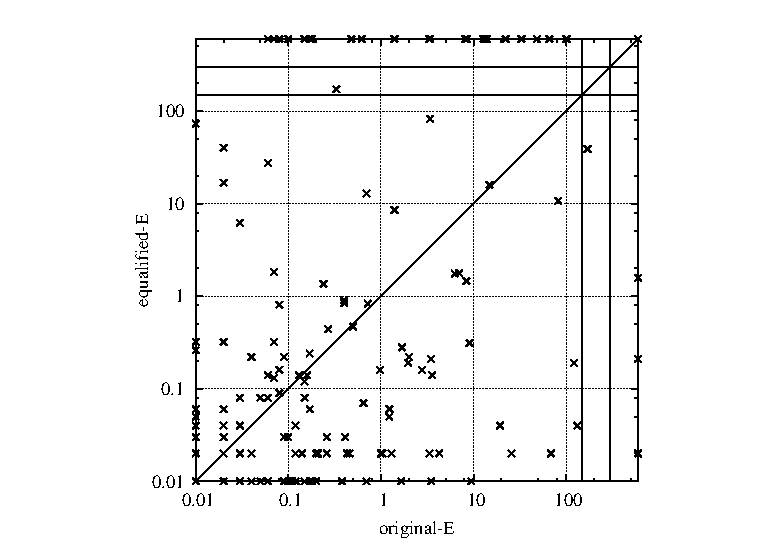
\includegraphics[scale=0.65,trim=10mm 00mm 20mm 0mm]{Plots/Equalified/E/test_original_e_equalified_e_300.eps}
%\includegraphics[scale=0.22]{Plots/Equalified/E/}
%\begin{figure}[t]
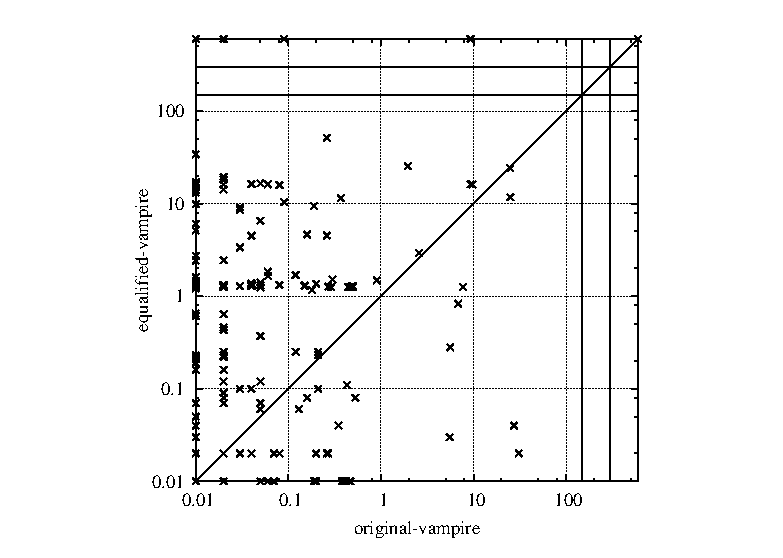
\includegraphics[scale=0.65,trim=10mm 0mm 20mm 0mm]{Plots/Equalified/Vampire/test_original_vampire_equalified_vampire_300.eps}\\
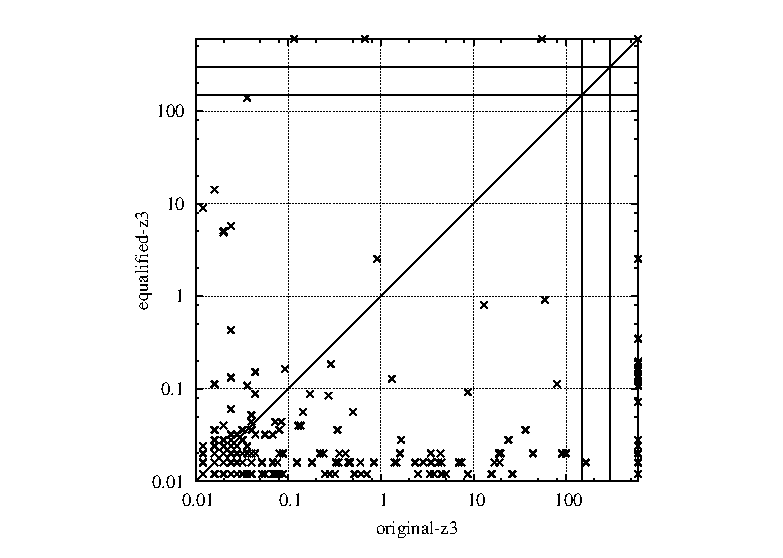
\includegraphics[scale=0.65,trim=10mm 0mm 20mm 0mm]{Plots/Equalified/Z3/test_original_z3_equalified_z3_300.eps}
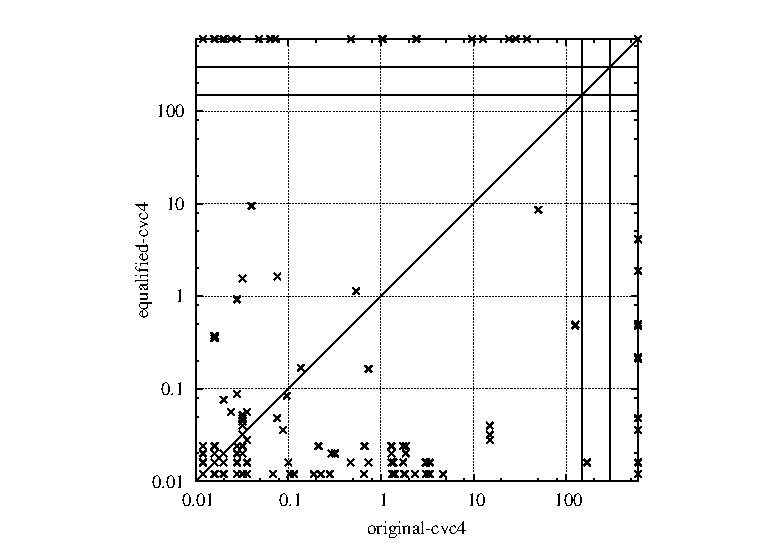
\includegraphics[scale=0.65,trim=10mm 0mm 20mm 0mm]{Plots/Equalified/CVC4/test_original_cvc4_equalified_cvc4_300.eps}
\end{center}
\caption{The time taken to solve problems, with and without equalification, using E, Vampire, Z3 and CVC4 }
%\includegraphics[scale=0.22]{Plots/Equalified/E/}
%\end{figure}
\label{fig:e_equalified}
\end{figure}

\subsection{Equivalence relations}

Equivalence relations were present in 430 of the test problems. The majority of these problems appear in the GEO and SYN categories. Interestingly, among these 430 problems, there are only 23 problems whose equivalence relations are axiomatized with transitivity axioms. The remaining 407 problems axiomatize equivalence relations with euclidean and reflexivity axioms, as discussed in section \ref{sec:discovery}. The number of equivalence relations in each problem ranges from 1 to 40, where problems with many equivalence relations all come from the SYN category. There is no clear correspondence between the number of equivalence relations in a problem and the performance of the prover prior to and after the transformation. 

\paragraph{Equalification}
As can be seen in Fig. \ref{fig:overview}, equalification performs very well with Z3, and somewhat well with CVC4, while it worsens the results of the resolution based provers, which already performed well on the original problems. %TODO : Koen - why may this be? 
Using a time slicing strategy, which runs the prover on the original problem for half the time and on the transformed problem for the second half, solves a strict superset of problems than the original for all of the theorem provers used in the evaluation. Fig. \ref{fig:e_equalified} shows in more detail the effect on solving times for the different theorem provers.
%TODO: for the camera ready version we should make the time slicing squares the biggest possible size.

%TODO KOEN: i don't like the word treatment. it sounds like a cream you put on your skin.

\paragraph{Pequalification}
In 181 of the test problems, relations that are transitive and symmetric, but not reflexive, were found. The majority of these problems are in the CAT and FLD categories of TPTP. All of the tested theorem provers perform worse on these problems compared to the problems with true equivalence relations. This is also the case after performing pequalification. Pequalification turns out to be particularly bad for E, which solves 34 fewer problems after the transformation. Pequalification makes Z3 perform only slightly better and Vampire and CVC4 slightly worse. 
When the differences to the performance is small, it is hard to know if the effect is due to the new axiomatisation, or to other reasons. For example, we have observed that simply shuffling the axioms of a theory can cause the results to deviate in a similar way. 
%TODO Koen can we say anything more here?

\subsection{Total orders}
Total orders were found in 328 problems. The majority are in the SWV category, and the remaining in HWV, LDA and NUM.  In 77 of the problems, the total order is positively axiomatized, and in the other 251 problems it is negative (and thus axiomatized as a strict total order). There is never more than one order present in any of the problems. 

\begin{figure}[t]
%\includegraphics[scale=0.40,trim=20mm 00mm 30mm 0mm]{Plots/Ordified/E/test_original_e_ordified_e_300.eps}
%\includegraphics[scale=0.22]{Plots/Equalified/E/}
%\begin{figure}[t]
\begin{center}
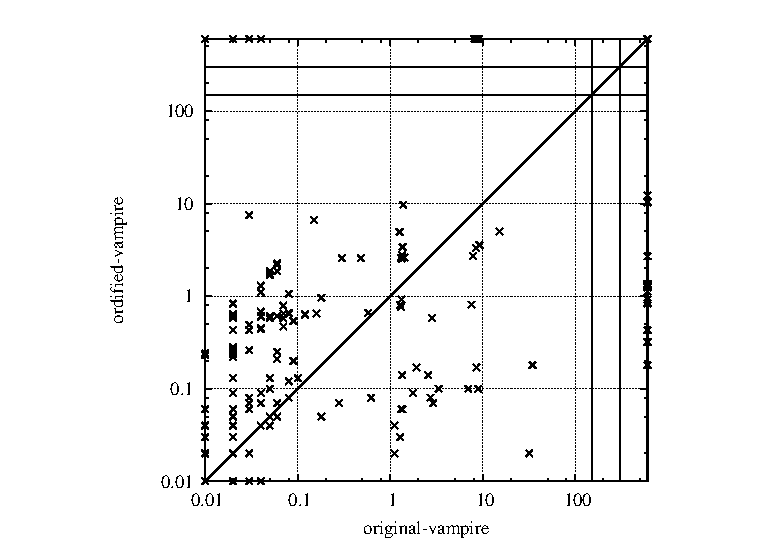
\includegraphics[scale=0.55,trim=20mm 0mm 30mm 0mm]{Plots/Ordified/Vampire/test_original_vampire_ordified_vampire_300.eps}
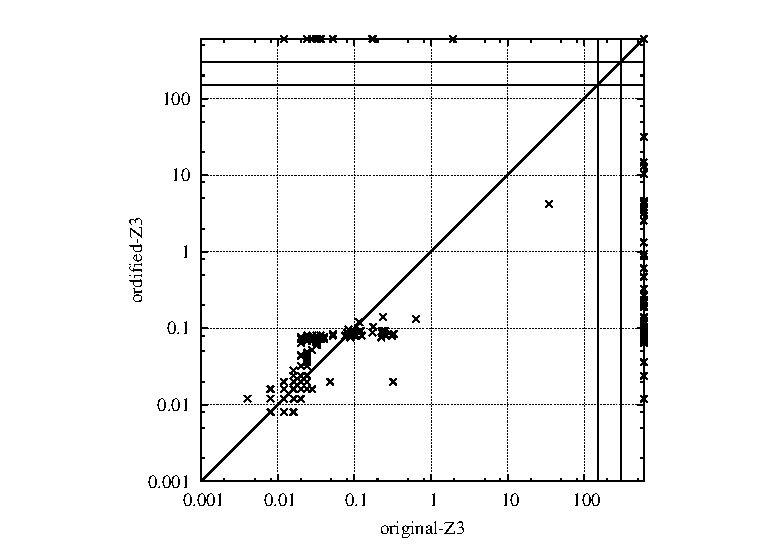
\includegraphics[scale=0.55,trim=7mm 0mm 30mm 0mm]{Plots/Ordified/Z3/test_original_Z3_ordified_Z3_300.eps}
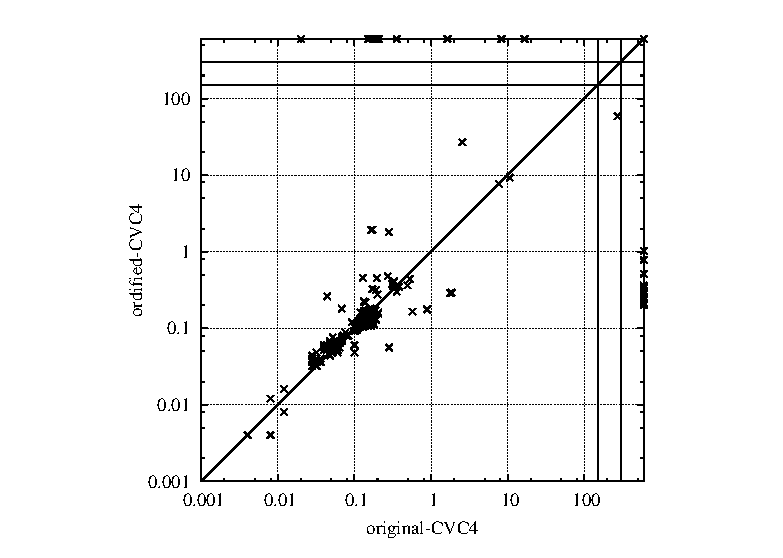
\includegraphics[scale=0.55,trim=7mm 0mm 40mm 0mm]{Plots/Ordified/CVC4/test_original_CVC4_ordified_cvc4_300.eps}
\end{center}
%\includegraphics[scale=0.22]{Plots/Equalified/E/}
\caption{Effects of ordification, using Vampire, Z3 and CVC4 }
\label{fig:ordified}
\end{figure}

\paragraph{Ordification}
For each of the problems, we ran the theorem provers with built-in support for arithmetic on the problems before and after applying ordification. Vampire was run on a version in TFF format \cite{TFF}, and Z3 and CVC4 on a version in SMT format \cite{SMT-LIB}. The original problems were also transformed into TFF and SMT in order to achieve a relevant comparison. Ordification performs well for Z3, while for Vampire and CVC4 it is good for some problems and bad for some.
Fig.\ \ref{fig:ordified} shows how solving times are affected, and the diagrams also show great potential for time slicing, in particular for Vampire and Z3.

\paragraph{Hard problems solved using Ordification}
After Ordification, 15 problems, all from the SWV category, with rating 1.0 are solved. (SWV004-1, SWV035+1, SWV040+1, SWV044+1, SWV049+1, SWV079+1, SWV100+1, SWV101+1, SWV108+1, SWV110+1, SWV113+1, SWV118+1, SWV120+1, SWV124+1, SWV130+1) Vampire and Z3 each solve 14 hard problems and CVC4 solves 13 of them. Rating 1.0 means that no known current theorem prover solves the problem in reasonable time. One problem (SWV004-1) is even categorized as Unknown, which means that no prover has ever solved it. After ordification, all three provers were able to solve it in less than a second.

\paragraph{Maxification}
Maxification, the second possible treatment of total orders, turned out to be disadvantageous to E and Z3, while having very little effect on Vampire and CVC4 (see Fig.\ \ref{fig:overview}).
%TODO Koen what may be a reason for this?

%\begin{figure}[t]
%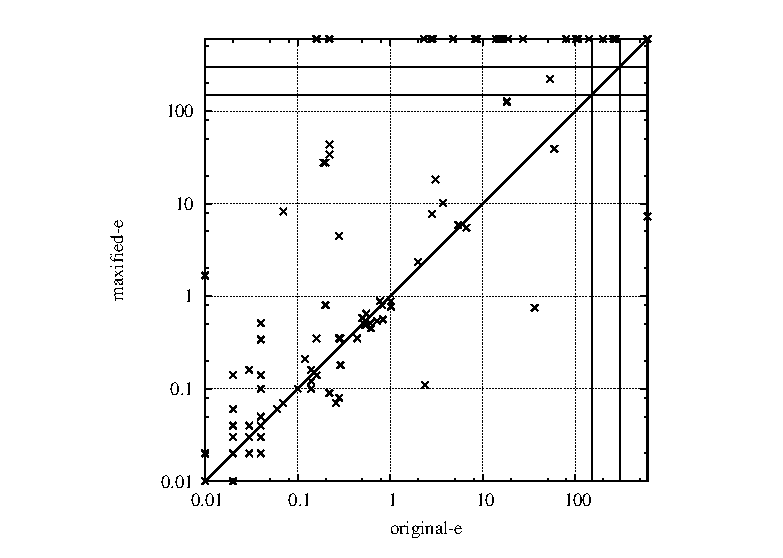
\includegraphics[scale=0.70,trim=10mm 00mm 20mm 0mm]{Plots/Maxified/E/test_original_e_maxified_e_300.eps}
%\includegraphics[scale=0.22]{Plots/Equalified/E/}
%\begin{figure}[t]
%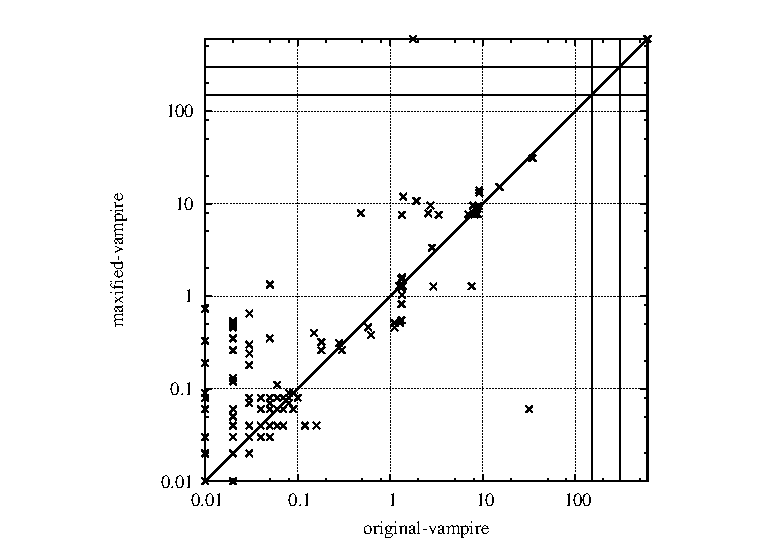
\includegraphics[scale=0.70,trim=10mm 0mm 20mm 0mm]{Plots/Maxified/Vampire/test_original_vampire_maxified_vampire_300.eps}\\
%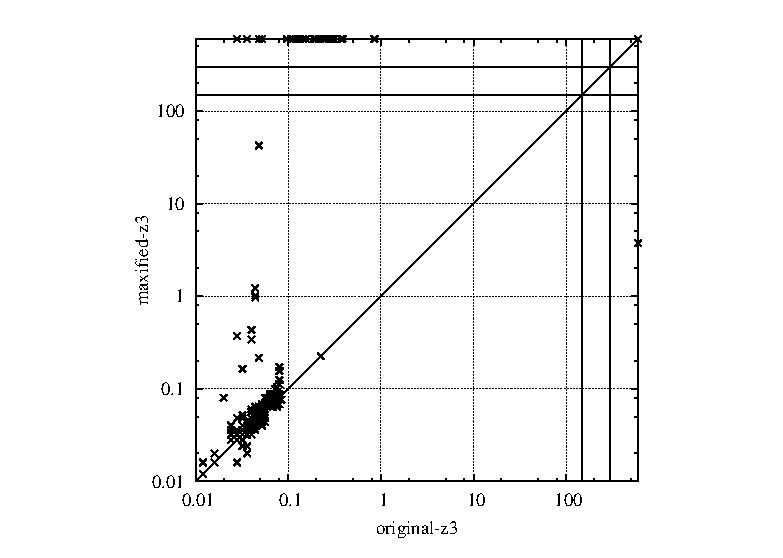
\includegraphics[scale=0.70,trim=10mm 0mm 20mm 0mm]{Plots/Maxified/Z3/test_original_z3_maxified_z3_300.eps} 
%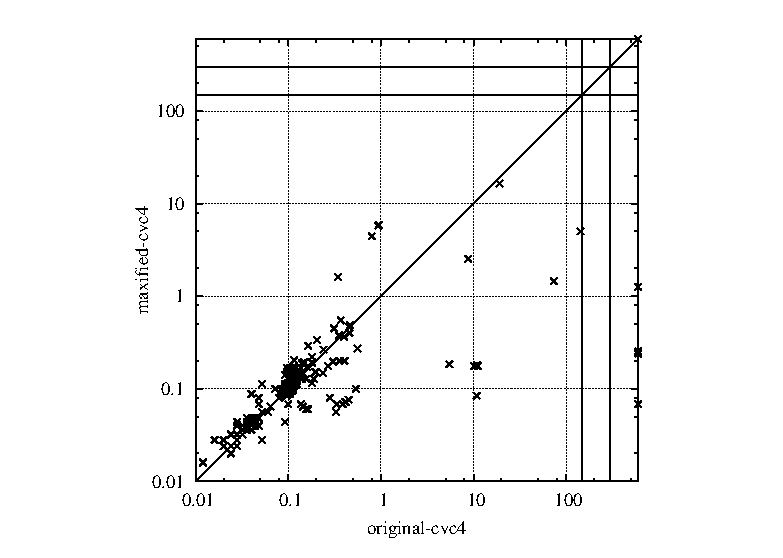
\includegraphics[scale=0.70,trim=10mm 0mm 20mm 0mm]{Plots/Maxified/CVC4/test_original_cvc4_maxified_cvc4_300.eps}
%\caption{Effects of maxification, using E, Vampire, Z3 and CVC4 }
%\includegraphics[scale=0.22]{Plots/Equalified/E/}
%\end{figure}
%\end{figure}


\subsection{Transitive and Reflexive relations}
573 test problems include relations that are transitive and reflexive, excluding equivalence relations and total orders. In all of them, transitivity occurs syntactically as an axiom. The problems come from a variety of categories, but a vast majority are in SET, SEU and SWV.  Only about half of the original problems were solved by each theorem prover, which may indicate that transitivity axioms are difficult for current theorem provers to deal with.  We evaluate the performance of the theorem provers before and after transification. Problems that include equivalence relations and total orders are excluded, as the corresponding methods equalification and ordification give better results and should be preferred. Vampire benefits the most from transification, and solves 32 new problems after the transformation, while 10 previously solvable problems become unsolvable within the time limit. For E, the effect of transification is almost exclusively negative.
%TODO what to write here?? 
Vampire also has a significantly worse performance than E overall on the original problems that include relations that are transitive and reflexive.
Both Z3 and CVC4 perform worse after the transformation, but time slicing can be a good way to improve the results. 

%TODO KOEN: who uses chaining? is Vampire better on transified problems because it doesn't use chaining?

\begin{figure}[t]
\begin{center}
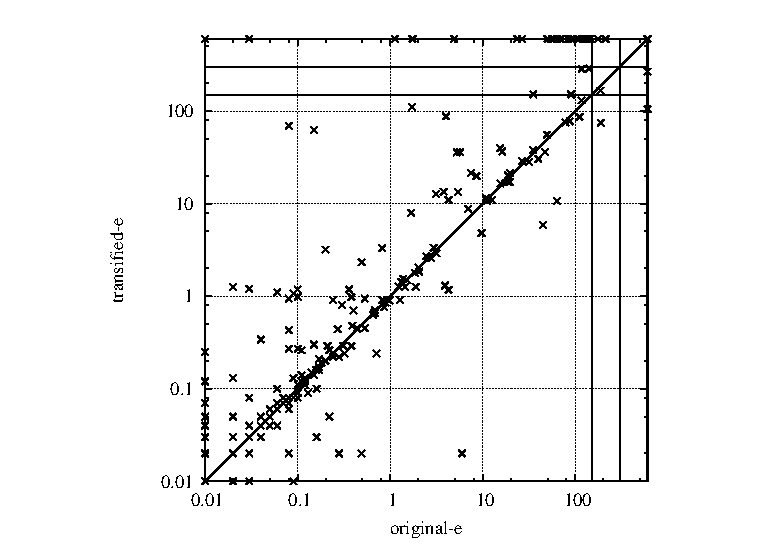
\includegraphics[scale=0.65,trim=10mm 00mm 20mm 0mm]{Plots/OnlyTransify/E/test_original_e_transified_e_300.eps}
%\includegraphics[scale=0.22]{Plots/Equalified/E/}
%\begin{figure}[t]
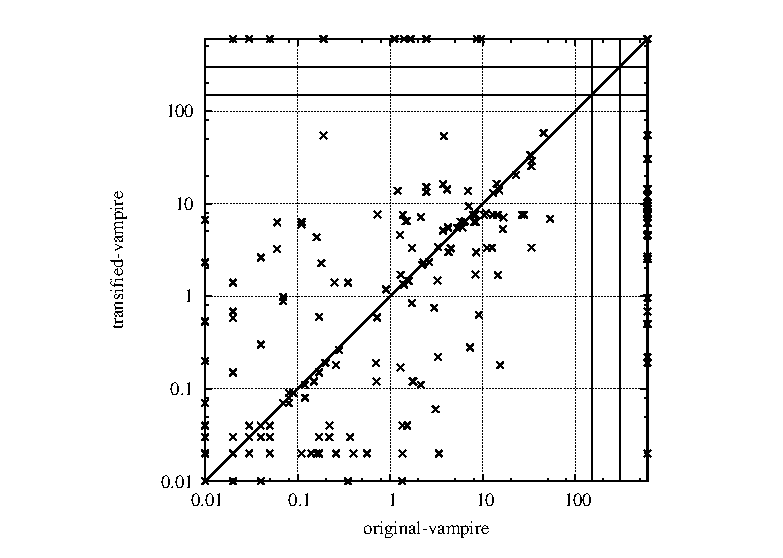
\includegraphics[scale=0.65,trim=10mm 0mm 20mm 0mm]{Plots/OnlyTransify/Vampire/test_original_vampire_transified_vampire_300.eps}\\
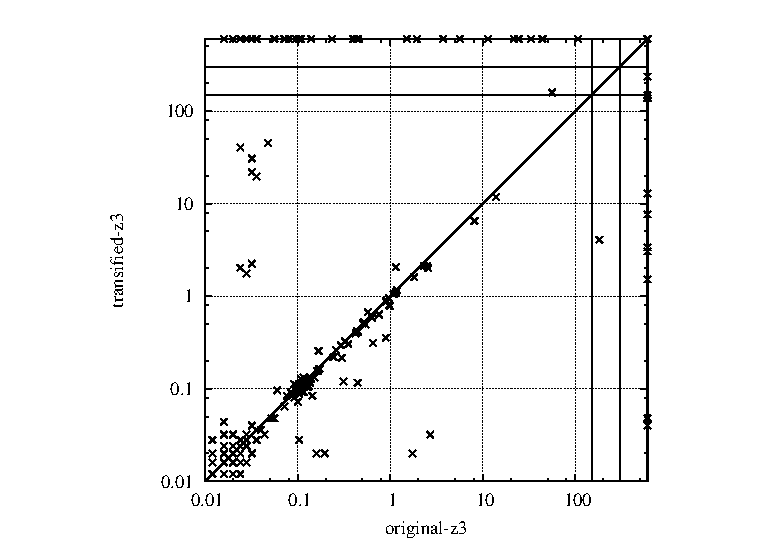
\includegraphics[scale=0.65,trim=10mm 0mm 20mm 0mm]{Plots/OnlyTransify/Z3/test_original_z3_transified_z3_300.eps} 
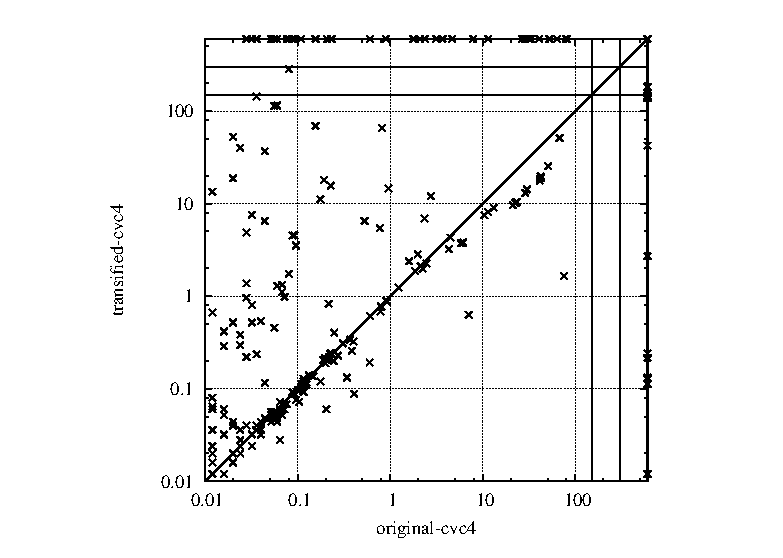
\includegraphics[scale=0.65,trim=10mm 0mm 20mm 0mm]{Plots/OnlyTransify/CVC4/test_original_cvc4_transified_cvc4_300.eps}
\end{center}
\caption{Effects of transification, using E, Vampire, Z3 and CVC4 }
%\includegraphics[scale=0.22]{Plots/Equalified/E/}
%\end{figure}
\end{figure}


\paragraph{Hard problems solved using Transification}
After transification, two new problems with rating 1.0 are solved, both by Vampire (SEU322+2 and SEU372+2).

\paragraph{Equalification and Transification}
Since all equivalence relations are transitive and reflexive, the method for transification works also on equivalence relations. Comparing the two methods on the 430 problems with equivalence relations, we concluded that equalification and transification work equally bad for E, Vampire and CVC4. Both transification and equalification improve the results for Z3, but equalification does so significantly. 

\paragraph{Ordification and Transification}
We compared ordification and transification on the 328 problems containing total orders. Transification seems to make these problems generally more difficult for theorem provers to solve, while ordification instead improved the results on many of the problems.  Transification makes the theorem prover perform worse on these problems also for E, which cannot make use of ordification since it does not provide support for arithmetic.

%(equalification: win 50 lose 3, transification: win 46, lose 27)

% ------------------------------------------------------------------------------
% - discussion and related work
% - conclusions and future work

\section{Discussion, Conclusions, and Future Work}

We have presented 5 transformations that can be applied to theories with certain transitive relations: equalification, pequalification, transification, ordification, and maxification. We have also created a method for syntactic discovery of binary relations where these transformations are applicable.

For users of reasoning tools that create their own theories, it is clear that they should consider using one of the proposed alternative treatments when writing theories. For all of our methods, there are existing theories for which some provers performed better on these theories than others. In particular, for transification and ordification, there exist 17 TPTP problems that are now solvable that weren't previously.

For implementers of reasoning tools, our conclusions are less clear. For some combinations of treatments and provers (such as transification for Vampire, and equalification for Z3), overall results are clearly better, and we would thus recommend these treatments as preprocessors for these provers. Some more combinations of treatments and provers lend themselves to a time slicing strategy that can solve strictly more problems, and could thusly be integrated in a natural way in provers that already have the time slicing machinery in place.

\paragraph{Related Work} Chaining \cite{chaining} is a family of methods that limit the use of transitivity-like axioms in proofs by only allowing certain chains of them to occur in proofs. The result is a complete proof system that avoids the derivation of unnecessary consequences of transitivity. However, chaining is not implemented in any of the reasoning tools we considered for this paper. In personal communication with some of the authors, chaining-like techniques have not been deemed important enough to be considered for implementation, and their preliminary experimental results were mostly negative.

\paragraph{Future Work} There is a lot of room for improvements and other future work. There are many other relations that are more or less common that could benefit from an alternative treatment like the transformations described in this paper. In particular, maxification seems to be an idea that could be applied to binary relations that are weaker than total orders, which may make this treatment more effective. But there are also other, non-transitive relations that are of interest.

Ordification uses total orders as the base-transformation, and treats strict total orders as negated total orders. We would like to investigate more in which cases it may be beneficial to treat strict total orders differently from total orders, and when to use $<$ on \ensuremath{\mathbb{R}} instead of \ensuremath{\leq }.

We would also like to investigate the effect of our transformations on Satisfiable and CounterSatisfiable problems. What would be the effect on finite model finders? Some transformations change the number of variables per clause, which will influence the performance of finite model finders. What happens to saturation-based tools? Is it easier or harder to saturate a problem after transformation? Evaluating these questions is hard, because we did not find many satisfiable problems in the TPTP that contained relevant relations (see Fig.\ \ref{fig:occurs2}). Instead, we considered using Unsatisfiable problems, and measuring the time it takes to show the absence of models up to a certain size.

There are other kinds of relations than binary relations. For example, we can have an ternary relation that behaves as an equivalence relation in its 2nd and 3rd argument. An alternative treatment of this relation would be to introduce a binary function symbol \ensuremath{rep}. We do not know whether or not this occurs often, and if it is a good idea to treat higher-arity relational symbols specially in this way.

Lastly, we would like to look at how these ideas could be used inside a theorem prover; as soon as the prover discovers that a relation is an equivalence relation or a total order, one of our transformations could be applied, on the fly. The details of how to do this remain to be investigated.

% ------------------------------------------------------------------------------
% - references

\bibliographystyle{plain}
\bibliography{main}

\end{document}

